%%
% Copyright (c) 2017 - 2025, Pascal Wagler;
% Copyright (c) 2014 - 2025, John MacFarlane
%
% All rights reserved.
%
% Redistribution and use in source and binary forms, with or without
% modification, are permitted provided that the following conditions
% are met:
%
% - Redistributions of source code must retain the above copyright
% notice, this list of conditions and the following disclaimer.
%
% - Redistributions in binary form must reproduce the above copyright
% notice, this list of conditions and the following disclaimer in the
% documentation and/or other materials provided with the distribution.
%
% - Neither the name of John MacFarlane nor the names of other
% contributors may be used to endorse or promote products derived
% from this software without specific prior written permission.
%
% THIS SOFTWARE IS PROVIDED BY THE COPYRIGHT HOLDERS AND CONTRIBUTORS
% "AS IS" AND ANY EXPRESS OR IMPLIED WARRANTIES, INCLUDING, BUT NOT
% LIMITED TO, THE IMPLIED WARRANTIES OF MERCHANTABILITY AND FITNESS
% FOR A PARTICULAR PURPOSE ARE DISCLAIMED. IN NO EVENT SHALL THE
% COPYRIGHT OWNER OR CONTRIBUTORS BE LIABLE FOR ANY DIRECT, INDIRECT,
% INCIDENTAL, SPECIAL, EXEMPLARY, OR CONSEQUENTIAL DAMAGES (INCLUDING,
% BUT NOT LIMITED TO, PROCUREMENT OF SUBSTITUTE GOODS OR SERVICES;
% LOSS OF USE, DATA, OR PROFITS; OR BUSINESS INTERRUPTION) HOWEVER
% CAUSED AND ON ANY THEORY OF LIABILITY, WHETHER IN CONTRACT, STRICT
% LIABILITY, OR TORT (INCLUDING NEGLIGENCE OR OTHERWISE) ARISING IN
% ANY WAY OUT OF THE USE OF THIS SOFTWARE, EVEN IF ADVISED OF THE
% POSSIBILITY OF SUCH DAMAGE.
%%

%%
% This is the Eisvogel pandoc LaTeX template.
%
% For usage information and examples visit the official GitHub page:
% https://github.com/Wandmalfarbe/pandoc-latex-template
%%
% Options for packages loaded elsewhere
\PassOptionsToPackage{unicode}{hyperref}
\PassOptionsToPackage{hyphens}{url}
\PassOptionsToPackage{dvipsnames,svgnames,x11names,table}{xcolor}
\documentclass[
  american,
  11pt,
  letterpaper,
  oneside  ,captions=tableheading
]{scrartcl}
\usepackage{xcolor}
\usepackage[margin=1in]{geometry}
\usepackage{amsmath,amssymb}

% add backlinks to footnote references, cf. https://tex.stackexchange.com/questions/302266/make-footnote-clickable-both-ways
\usepackage{footnotebackref}
\setcounter{secnumdepth}{5}
\usepackage{iftex}
\ifPDFTeX
  \usepackage[T1]{fontenc}
  \usepackage[utf8]{inputenc}
  \usepackage{textcomp} % provide euro and other symbols
\else % if luatex or xetex
  \usepackage{unicode-math} % this also loads fontspec
  \defaultfontfeatures{Scale=MatchLowercase}
  \defaultfontfeatures[\rmfamily]{Ligatures=TeX,Scale=1}
\fi
\usepackage{lmodern}
\ifPDFTeX\else
  % xetex/luatex font selection
  \setmainfont[]{DejaVu Serif}
  \setsansfont[]{DejaVu Sans}
  \setmonofont[]{DejaVu Sans Mono}
\fi
% Use upquote if available, for straight quotes in verbatim environments
\IfFileExists{upquote.sty}{\usepackage{upquote}}{}
\IfFileExists{microtype.sty}{% use microtype if available
  \usepackage[]{microtype}
  \UseMicrotypeSet[protrusion]{basicmath} % disable protrusion for tt fonts
}{}

\usepackage{setspace}
\makeatletter
\@ifundefined{KOMAClassName}{% if non-KOMA class
  \IfFileExists{parskip.sty}{%
    \usepackage{parskip}
  }{% else
    \setlength{\parindent}{0pt}
    \setlength{\parskip}{6pt plus 2pt minus 1pt}}
}{% if KOMA class
  \KOMAoptions{parskip=half}}
\makeatother
\usepackage{listings}
\newcommand{\passthrough}[1]{#1}
\lstset{defaultdialect=[5.3]Lua}
\lstset{defaultdialect=[x86masm]Assembler}
\usepackage{etoolbox}
\BeforeBeginEnvironment{lstlisting}{\par\noindent\begin{minipage}{\linewidth}}
\AfterEndEnvironment{lstlisting}{\end{minipage}\par\addvspace{\topskip}}
\usepackage{longtable,booktabs,array}
\newcounter{none} % for unnumbered tables
\usepackage{calc} % for calculating minipage widths
% Correct order of tables after \paragraph or \subparagraph
\usepackage{etoolbox}
\makeatletter
\patchcmd\longtable{\par}{\if@noskipsec\mbox{}\fi\par}{}{}
\makeatother
% Allow footnotes in longtable head/foot
\IfFileExists{footnotehyper.sty}{\usepackage{footnotehyper}}{\usepackage{footnote}}
\makesavenoteenv{longtable}
% definitions for citeproc citations
\NewDocumentCommand\citeproctext{}{}
\NewDocumentCommand\citeproc{mm}{%
  \begingroup\def\citeproctext{#2}\cite{#1}\endgroup}
\makeatletter
 % allow citations to break across lines
 \let\@cite@ofmt\@firstofone
 % avoid brackets around text for \cite:
 \def\@biblabel#1{}
 \def\@cite#1#2{{#1\if@tempswa , #2\fi}}
\makeatother
\newlength{\cslhangindent}
\setlength{\cslhangindent}{1.5em}
\newlength{\csllabelwidth}
\setlength{\csllabelwidth}{3em}
\newenvironment{CSLReferences}[2] % #1 hanging-indent, #2 entry-spacing
 {\begin{list}{}{%
  \setlength{\itemindent}{0pt}
  \setlength{\leftmargin}{0pt}
  \setlength{\parsep}{0pt}
  % turn on hanging indent if param 1 is 1
  \ifodd #1
   \setlength{\leftmargin}{\cslhangindent}
   \setlength{\itemindent}{-1\cslhangindent}
  \fi
  % set entry spacing
  \setlength{\itemsep}{#2\baselineskip}}}
 {\end{list}}
\usepackage{calc}
\newcommand{\CSLBlock}[1]{\hfill\break\parbox[t]{\linewidth}{\strut\ignorespaces#1\strut}}
\newcommand{\CSLLeftMargin}[1]{\parbox[t]{\csllabelwidth}{\strut#1\strut}}
\newcommand{\CSLRightInline}[1]{\parbox[t]{\linewidth - \csllabelwidth}{\strut#1\strut}}
\newcommand{\CSLIndent}[1]{\hspace{\cslhangindent}#1}
\ifLuaTeX
\usepackage[bidi=basic,shorthands=off]{babel}
\else
\usepackage[bidi=default,shorthands=off]{babel}
\fi
\ifPDFTeX
\else
\babelfont{rm}[]{DejaVu Serif}
\fi
\ifLuaTeX
  \usepackage{selnolig} % disable illegal ligatures
\fi
\setlength{\emergencystretch}{3em} % prevent overfull lines
\providecommand{\tightlist}{%
  \setlength{\itemsep}{0pt}\setlength{\parskip}{0pt}}
\usepackage{graphicx}
\usepackage{xurl}
\usepackage{rotating}
\usepackage{booktabs}
\usepackage{bookmark}
\IfFileExists{xurl.sty}{\usepackage{xurl}}{} % add URL line breaks if available
\urlstyle{same}
\definecolor{default-linkcolor}{HTML}{A50000}
\definecolor{default-filecolor}{HTML}{A50000}
\definecolor{default-citecolor}{HTML}{4077C0}
\definecolor{default-urlcolor}{HTML}{4077C0}

\hypersetup{
  pdftitle={Healthcare Analytics Challenges: A Three-Pillar Framework Connecting Analytics Maturity, Workforce Agility, and Technical Enablement},
  pdfauthor={Samuel T Harrold, Yuimedi},
  pdflang={en-US},
  pdfkeywords={healthcare analytics, healthcare informatics, analytical
framework, analytics maturity, workforce turnover, institutional
memory, text-to-SQL, natural language processing, knowledge
portal, conversational AI},
  colorlinks=true,
  linkcolor={blue},
  filecolor={default-filecolor},
  citecolor={blue},
  urlcolor={blue},
  breaklinks=true,
  pdfcreator={LaTeX via pandoc with the Eisvogel template}}

\title{Healthcare Analytics Challenges: A Three-Pillar Framework
Connecting Analytics Maturity, Workforce Agility, and Technical
Enablement}
\author{Samuel T Harrold, Yuimedi}
\date{January 2026}


%
% for the background color of the title page
%
\usepackage{pagecolor}
\usepackage{afterpage}

%
% break urls
%
\PassOptionsToPackage{hyphens}{url}

%
% When using babel or polyglossia with biblatex, loading csquotes is recommended
% to ensure that quoted texts are typeset according to the rules of your main language.
%
\usepackage{csquotes}

%
% captions
%
\definecolor{caption-color}{HTML}{777777}
\usepackage[font={stretch=1.2}, textfont={color=caption-color}, position=top, skip=4mm, labelfont=bf, singlelinecheck=false, justification=raggedright]{caption}
\setcapindent{0em}

%
% blockquote
%
\definecolor{blockquote-border}{RGB}{221,221,221}
\definecolor{blockquote-text}{RGB}{119,119,119}
\usepackage{mdframed}
\newmdenv[rightline=false,bottomline=false,topline=false,linewidth=3pt,linecolor=blockquote-border,skipabove=\parskip]{customblockquote}
\renewenvironment{quote}{\begin{customblockquote}\list{}{\rightmargin=0em\leftmargin=0em}%
\item\relax\color{blockquote-text}\ignorespaces}{\unskip\unskip\endlist\end{customblockquote}}

%
% Source Sans Pro as the default font family
% Source Code Pro for monospace text
%
% 'default' option sets the default
% font family to Source Sans Pro, not \sfdefault.
%
% Note that the font has been officially renamed to `Source Sans 3`, and
% the version provided by the `sourcesanspro` package is slightly outdated.
% You can install the newer version locally and use it, for example, with
% `mainfont: "Source Sans 3"` in the YAML metadata (requires XeTeX or LuaTeX).
%
\ifnum 0\ifxetex 1\fi\ifluatex 1\fi=0 % if pdftex
    \usepackage[default]{sourcesanspro}
  \usepackage{sourcecodepro}
  \else % if not pdftex
    \fi

%
% heading color
%
\definecolor{heading-color}{RGB}{40,40,40}
% By default, the KOMA-Script classes will typeset sectioning headings in
% sans-serif. Use the normal body font for headings.
\addtokomafont{disposition}{\normalfont\color{heading-color}\bfseries}

%
% variables for title, author and date
%
\usepackage{titling}
\title{Healthcare Analytics Challenges: A Three-Pillar Framework
Connecting Analytics Maturity, Workforce Agility, and Technical
Enablement}
\author{Samuel T Harrold, Yuimedi}
\date{January 2026}

%
% tables
%

\definecolor{table-row-color}{HTML}{F5F5F5}
\definecolor{table-rule-color}{HTML}{999999}

%\arrayrulecolor{black!40}
\arrayrulecolor{table-rule-color}     % color of \toprule, \midrule, \bottomrule
\setlength\heavyrulewidth{0.3ex}      % thickness of \toprule, \bottomrule
\renewcommand{\arraystretch}{1.3}     % spacing (padding)


%
% remove paragraph indentation
%
\setlength{\parindent}{0pt}
\setlength{\parskip}{6pt plus 2pt minus 1pt}
\setlength{\emergencystretch}{3em}  % prevent overfull lines

%
%
% Listings
%
%


%
% general listing colors
%
\definecolor{listing-background}{HTML}{F7F7F7}
\definecolor{listing-rule}{HTML}{B3B2B3}
\definecolor{listing-numbers}{HTML}{B3B2B3}
\definecolor{listing-text-color}{HTML}{000000}
\definecolor{listing-keyword}{HTML}{435489}
\definecolor{listing-keyword-2}{HTML}{1284CA} % additional keywords
\definecolor{listing-keyword-3}{HTML}{9137CB} % additional keywords
\definecolor{listing-identifier}{HTML}{435489}
\definecolor{listing-string}{HTML}{00999A}
\definecolor{listing-comment}{HTML}{8E8E8E}

\lstdefinestyle{eisvogel_listing_style}{
  language         = java,
  numbers          = left,
  xleftmargin      = 2.7em,
  framexleftmargin = 2.5em,
  backgroundcolor  = \color{listing-background},
  basicstyle       = \color{listing-text-color}\linespread{1.0}%
                      \lst@ifdisplaystyle%
                      \small%
                      \fi\ttfamily{},
  breaklines       = true,
  frame            = single,
  framesep         = 0.19em,
  rulecolor        = \color{listing-rule},
  frameround       = ffff,
  tabsize          = 4,
  numberstyle      = \color{listing-numbers},
  aboveskip        = 1.0em,
  belowskip        = 0.1em,
  abovecaptionskip = 0em,
  belowcaptionskip = 1.0em,
  keywordstyle     = {\color{listing-keyword}\bfseries},
  keywordstyle     = {[2]\color{listing-keyword-2}\bfseries},
  keywordstyle     = {[3]\color{listing-keyword-3}\bfseries\itshape},
  sensitive        = true,
  identifierstyle  = \color{listing-identifier},
  commentstyle     = \color{listing-comment},
  stringstyle      = \color{listing-string},
  showstringspaces = false,
  escapeinside     = {/*@}{@*/}, % Allow LaTeX inside these special comments
  literate         =
  {á}{{\'a}}1 {é}{{\'e}}1 {í}{{\'i}}1 {ó}{{\'o}}1 {ú}{{\'u}}1
  {Á}{{\'A}}1 {É}{{\'E}}1 {Í}{{\'I}}1 {Ó}{{\'O}}1 {Ú}{{\'U}}1
  {à}{{\`a}}1 {è}{{\`e}}1 {ì}{{\`i}}1 {ò}{{\`o}}1 {ù}{{\`u}}1
  {À}{{\`A}}1 {È}{{\`E}}1 {Ì}{{\`I}}1 {Ò}{{\`O}}1 {Ù}{{\`U}}1
  {ä}{{\"a}}1 {ë}{{\"e}}1 {ï}{{\"i}}1 {ö}{{\"o}}1 {ü}{{\"u}}1
  {Ä}{{\"A}}1 {Ë}{{\"E}}1 {Ï}{{\"I}}1 {Ö}{{\"O}}1 {Ü}{{\"U}}1
  {â}{{\^a}}1 {ê}{{\^e}}1 {î}{{\^i}}1 {ô}{{\^o}}1 {û}{{\^u}}1
  {Â}{{\^A}}1 {Ê}{{\^E}}1 {Î}{{\^I}}1 {Ô}{{\^O}}1 {Û}{{\^U}}1
  {œ}{{\oe}}1 {Œ}{{\OE}}1 {æ}{{\ae}}1 {Æ}{{\AE}}1 {ß}{{\ss}}1
  {ç}{{\c c}}1 {Ç}{{\c C}}1 {ø}{{\o}}1 {å}{{\r a}}1 {Å}{{\r A}}1
  {€}{{\EUR}}1 {£}{{\pounds}}1 {«}{{\guillemotleft}}1
  {»}{{\guillemotright}}1 {ñ}{{\~n}}1 {Ñ}{{\~N}}1 {¿}{{?`}}1
  {…}{{\ldots}}1 {≥}{{>=}}1 {≤}{{<=}}1 {„}{{\glqq}}1 {“}{{\grqq}}1
  {”}{{''}}1
}
\lstset{style=eisvogel_listing_style}

%
% Java (Java SE 12, 2019-06-22)
%
\lstdefinelanguage{Java}{
  morekeywords={
    % normal keywords (without data types)
    abstract,assert,break,case,catch,class,continue,default,
    do,else,enum,exports,extends,final,finally,for,if,implements,
    import,instanceof,interface,module,native,new,package,private,
    protected,public,requires,return,static,strictfp,super,switch,
    synchronized,this,throw,throws,transient,try,volatile,while,
    % var is an identifier
    var
  },
  morekeywords={[2] % data types
    % primitive data types
    boolean,byte,char,double,float,int,long,short,
    % String
    String,
    % primitive wrapper types
    Boolean,Byte,Character,Double,Float,Integer,Long,Short
    % number types
    Number,AtomicInteger,AtomicLong,BigDecimal,BigInteger,DoubleAccumulator,DoubleAdder,LongAccumulator,LongAdder,Short,
    % other
    Object,Void,void
  },
  morekeywords={[3] % literals
    % reserved words for literal values
    null,true,false,
  },
  sensitive,
  morecomment  = [l]//,
  morecomment  = [s]{/*}{*/},
  morecomment  = [s]{/**}{*/},
  morestring   = [b]",
  morestring   = [b]',
}

\lstdefinelanguage{XML}{
  morestring      = [b]",
  moredelim       = [s][\bfseries\color{listing-keyword}]{<}{\ },
  moredelim       = [s][\bfseries\color{listing-keyword}]{</}{>},
  moredelim       = [l][\bfseries\color{listing-keyword}]{/>},
  moredelim       = [l][\bfseries\color{listing-keyword}]{>},
  morecomment     = [s]{<?}{?>},
  morecomment     = [s]{<!--}{-->},
  commentstyle    = \color{listing-comment},
  stringstyle     = \color{listing-string},
  identifierstyle = \color{listing-identifier}
}

%
% header and footer
%
\usepackage[headsepline,footsepline]{scrlayer-scrpage}

\newpairofpagestyles{eisvogel-header-footer}{
  \clearpairofpagestyles
  \ihead*{Healthcare Analytics Challenges}
  \chead*{}
  \ohead*{January 2026}
  \ifoot*{\hspace{0pt}}
  \cfoot*{\thepage}
  \ofoot*{\hspace{0pt}}
  \addtokomafont{pageheadfoot}{\upshape}
}
\pagestyle{eisvogel-header-footer}



%
% Define watermark
%

\begin{document}

\begin{titlepage}
\newgeometry{left=6cm}
\definecolor{titlepage-color}{HTML}{FFFFFF}
\newpagecolor{titlepage-color}\afterpage{\restorepagecolor}
\newcommand{\colorRule}[3][black]{\textcolor[HTML]{#1}{\rule{#2}{#3}}}
\begin{flushleft}
\noindent
\\[-1em]
\color[HTML]{000000}
\makebox[0pt][l]{\colorRule[000000]{1.3\textwidth}{2pt}}
\par
\noindent

{
  \setstretch{1.4}
  \vfill
  \noindent {\huge \textbf{\textsf{Healthcare Analytics Challenges: A
Three-Pillar Framework Connecting Analytics Maturity, Workforce Agility,
and Technical Enablement}}}
    \vskip 2em
  \noindent {\Large \textsf{Samuel T Harrold, Yuimedi}}
  \vfill
}


\textsf{January 2026}
\end{flushleft}
\end{titlepage}
\restoregeometry
\pagenumbering{arabic}

% don't generate the default title
% \maketitle
\begin{abstract}
\textbf{Background:} Healthcare organizations face three interconnected
challenges: low analytics maturity, with only 39 organizations globally
having achieved HIMSS AMAM Stage 6-7; systemic instability from high
leadership turnover (53\% of CIOs with \textless3 years tenure) and
persistent digital skills shortages; and technical barriers in natural
language to SQL generation. When these challenges interact, they create
institutional memory loss that threatens data-driven healthcare
transformation.

\textbf{Objective:} This research develops a three-pillar analytical
framework connecting analytics maturity, workforce agility, and
technical enablement. The framework reveals how these capabilities
interconnect and compound each other.

\textbf{Methods:} We conducted a narrative literature review of
peer-reviewed studies and industry reports on natural language to SQL
(NL2SQL) generation, healthcare analytics maturity, and workforce
turnover. Grey literature was assessed using the AACODS checklist.
Evidence was synthesized through the three-pillar analytical framework
to examine how these challenges interconnect and compound.

\textbf{Results:} Healthcare-specific text-to-SQL benchmarks show
significant progress, though current models are ``not yet sufficiently
accurate for unsupervised use'' in clinical settings. Most healthcare
organizations remain at HIMSS AMAM Stages 0-3 with limited predictive
capabilities. Healthcare IT turnover significantly exceeds other IT
sectors, creating measurable institutional memory loss. The framework
reveals a compounding dynamic: low-maturity organizations experience
higher turnover, which degrades the institutional knowledge needed for
maturity advancement, while technical barriers prevent the capture of
expertise before it is lost.

\textbf{Conclusions:} We contribute a three-pillar analytical framework
synthesizing evidence on analytics maturity, workforce agility, and
technical enablement. The framework reveals a compounding effect: low
maturity accelerates turnover, which degrades maturity, and low
enablement prevents recovery. This analytical lens enables
organizational self-assessment and informs future research on
technological interventions, such as conversational AI platforms.
\end{abstract}


{
\setcounter{tocdepth}{3}
\tableofcontents
}
\setstretch{1.15}
\section{Introduction}\label{introduction}

\subsection{The Compounding Crisis in Healthcare
Analytics}\label{the-compounding-crisis-in-healthcare-analytics}

Healthcare organizations face three critical, interconnected challenges
that form a compounding crisis, collectively threatening their ability
to become data-driven enterprises. Unlike technology or financial
services, healthcare combines complex clinical workflows, extensive
regulatory requirements, and a workforce with limited technical training
but deep domain expertise
(\citeproc{ref-american2023}{\textbf{american2023?}}). This paper
introduces a three-pillar framework that examines how these challenges
interconnect and reinforce one another.

The framework follows a logical progression from observation to root
cause:

\begin{enumerate}
\def\labelenumi{\arabic{enumi}.}
\item
  \textbf{Pillar 1: Low Analytics Maturity (The Observation):} The most
  visible symptom is healthcare's struggle to advance its analytics
  capabilities. Despite massive investments in data infrastructure, most
  organizations remain at low maturity levels, unable to leverage their
  data for predictive or prescriptive insights.
\item
  \textbf{Pillar 2: Workforce Instability (The Cause):} This low
  maturity is not a static state but is actively driven by a systemic
  workforce crisis. High turnover at leadership, operational, and
  specialized levels creates a constant drain of institutional
  knowledge, preventing the accumulation of expertise required for
  maturity advancement.
\item
  \textbf{Pillar 3: Technical Barriers (The Root Mechanism):} The cycle
  is perpetuated by technical barriers that prevent organizations from
  capturing expertise before it is lost. The gap between clinical domain
  experts and the technical skills required for data access (e.g., SQL)
  creates a dependency on a small pool of specialists, making the system
  fragile and vulnerable to knowledge loss.
\end{enumerate}

This introduction will now examine the evidence for each of these
pillars in turn, establishing the foundation for the integrated
framework that is the central contribution of this paper.

\subsection{Pillar 1: Low Healthcare Analytics
Maturity}\label{pillar-1-low-healthcare-analytics-maturity}

The Healthcare Information Management Systems Society (HIMSS) Analytics
Maturity Assessment Model (AMAM) provides the industry standard for
measuring analytics capabilities. Recent assessments reveal a sobering
reality: as of late 2024, only 26 organizations worldwide had achieved
Stage 6 maturity, with merely 13 reaching Stage 7
(\citeproc{ref-himss2024}{\textbf{himss2024?}},\citeproc{ref-himss2024news}{\textbf{himss2024news?}}).
Despite this progress, the vast majority of organizations remain at
Stages 0-3, characterized by fragmented data, limited automated
reporting, and minimal predictive capabilities
(\citeproc{ref-himss2024}{\textbf{himss2024?}}). This low maturity
severely constrains evidence-based decision making.

\subsection{Pillar 2: Institutional Memory Loss from Workforce
Instability}\label{pillar-2-institutional-memory-loss-from-workforce-instability}

Healthcare faces an institutional memory crisis that has evolved from
simple turnover to systemic instability. This crisis unfolds at three
levels:

\begin{itemize}
\tightlist
\item
  \textbf{Strategic Level:} Leadership churn is acute, with 53\% of
  healthcare CIOs having a tenure of less than three years, leading to
  frequent shifts in analytics strategy
  (\citeproc{ref-wittkieffer2024}{\textbf{wittkieffer2024?}}).
\item
  \textbf{Operational Level:} 79\% of healthcare provider organizations
  report persistent shortages in ``Information and Digital Health''
  roles, leaving critical technical positions vacant
  (\citeproc{ref-himssworkforce2024}{\textbf{himssworkforce2024?}}).
\item
  \textbf{Foundational Level:} A 2025 analysis found that 55\% of public
  health informatics specialists intended to leave their positions,
  preventing the accumulation of the tacit knowledge needed to maintain
  analytics infrastructure
  (\citeproc{ref-rajamani2025}{\textbf{rajamani2025?}}).
\end{itemize}

This multi-layered churn creates a cascade of knowledge loss. When
experienced analysts leave, they take with them irreplaceable tacit
knowledge: business rules, data anomalies, and analytical context that
traditional documentation fails to capture. The challenge is not new; a
foundational 2004 study established that healthcare IT staff had the
lowest expected tenure for new hires among all IT sectors at just 2.9
years (\citeproc{ref-ang2004}{\textbf{ang2004?}}). That this
two-decade-old study remains a key benchmark is itself evidence of the
crisis: the industry is so unstable it has lost the ability to track its
own attrition.

\subsection{Pillar 3: Technical Barriers to Data
Access}\label{pillar-3-technical-barriers-to-data-access}

Against this backdrop of organizational immaturity and workforce
instability, technical barriers perpetuate the cycle. Accessing
healthcare insights requires navigating a complex technical landscape.
While the immediate barrier is often the ``technical skills
gap''---where clinical experts lack SQL expertise---this is merely the
surface of deeper challenges in \textbf{Semantic Interoperability} and
\textbf{Data Quality}
(\citeproc{ref-gal2019}{\textbf{gal2019?}},\citeproc{ref-zhang2024}{\textbf{zhang2024?}}).

In this context, Natural Language to SQL (NL2SQL) generation is not a
``magic bullet'' but a democratizing \textbf{Interface Layer} and a
\textbf{Governance Forcing Function}. For an AI system to translate a
natural language question into a correct SQL query, technical
prerequisites must be met: validated data models, explicit business
logic, and codified definitions. The AI interface forces the
organization to make this knowledge explicit, moving it from the minds
of a few experts into a durable, shared system. It provides a bridge
that allows non-technical domain experts to interact with data
\emph{alongside} these modernization efforts, unlocking value from
imperfect systems while broader interoperability efforts continue
(\citeproc{ref-anthropic2025}{\textbf{anthropic2025?}},\citeproc{ref-hendrix1978}{\textbf{hendrix1978?}},\citeproc{ref-ogunwole2023}{\textbf{ogunwole2023?}},\citeproc{ref-arora2025}{\textbf{arora2025?}}).

The implications of these three interconnected challenges are measurable
in both operational and clinical terms. When analytics barriers are
addressed, outcomes improve substantially: one Medicare ACO reduced
readmission rates from 24\% to 17.8\% and achieved \$1.6 million in cost
savings by implementing data analytics to overcome EHR fragmentation
(\citeproc{ref-latrella2024}{\textbf{latrella2024?}}). Yet, barriers
remain pervasive, with 68\% of healthcare organizations citing data
interoperability as the leading obstacle, followed by privacy concerns
(64\%) and insufficient staff training (59\%)
(\citeproc{ref-nashid2023}{\textbf{nashid2023?}}). Adoption of big data
analytics faces validated barriers including employee resistance to
change and lack of organizational readiness, which directly stall
data-driven initiatives
(\citeproc{ref-shahbaz2019}{\textbf{shahbaz2019?}},\citeproc{ref-kamble2019}{\textbf{kamble2019?}}).
Together, these three pillars represent a compounding cycle of
operational inefficiencies with demonstrated implications for healthcare
delivery.

\subsection{Objectives}\label{objectives}

This research aims to develop a framework for understanding healthcare's
interconnected analytics challenges. The specific objectives are as
follows:

\subsubsection{Primary Objective}\label{primary-objective}

Develop and validate a three-pillar analytical framework that explains
how analytics maturity, workforce agility, and technical enablement
interconnect and compound each other.

\subsubsection{Secondary Objectives}\label{secondary-objectives}

\begin{enumerate}
\def\labelenumi{\arabic{enumi}.}
\tightlist
\item
  \textbf{Synthesize current evidence} on natural language to SQL
  generation as a technical barrier.
\item
  \textbf{Document the extent} of analytics maturity challenges in
  healthcare organizations globally.
\item
  \textbf{Quantify the impact} of workforce turnover on institutional
  memory and analytics capabilities.
\item
  \textbf{Reveal interconnections} between the three pillars through
  evidence synthesis.
\item
  \textbf{Provide an assessment rubric} for organizational
  self-evaluation.
\end{enumerate}

\subsubsection{Non-Goals}\label{non-goals}

This research does not address:

\begin{itemize}
\tightlist
\item
  Specific vendor comparisons or product recommendations.
\item
  Implementation details for particular healthcare IT environments.
\item
  Regulatory compliance strategies for specific jurisdictions.
\item
  Technical architecture specifications for conversational AI systems.
\end{itemize}

\emph{Note: Analysis of market dynamics and structural factors
explaining why institution-specific analytics challenges persist is
within the scope of this paper. This market-level analysis provides
context for evaluating solution approaches and differs from product
comparisons, which would evaluate or recommend specific vendor
offerings.}

\subsection{Contributions}\label{contributions}

This paper makes the following contributions to the healthcare
informatics literature:

\begin{enumerate}
\def\labelenumi{\arabic{enumi}.}
\item
  \textbf{Three-Pillar Analytical Framework}: We synthesize evidence
  from three disconnected research domains---healthcare analytics
  maturity, workforce turnover, and natural language processing---into a
  unified analytical framework. This framework reveals how these
  challenges interconnect and compound each other: low maturity
  accelerates turnover, turnover degrades agility, and low technical
  enablement prevents recovery. The framework provides a lens for
  organizational self-assessment and research prioritization.
\item
  \textbf{Evidence Synthesis}: We document the current state of each
  pillar through a comprehensive literature review, providing healthcare
  organizations with consolidated evidence on analytics maturity
  benchmarks, the impact of workforce turnover, and NL2SQL technical
  capabilities.
\item
  \textbf{Illustrative Application}: Drawing on established knowledge
  management literature, we describe the validated query cycle as an
  example of how the framework can inform technology design. This
  concept addresses institutional memory loss through a six-step process
  that allows domain experts to validate and store queries, ensuring
  that knowledge persists independently of staff tenure. Figures 1 and 2
  illustrate this architecture and cycle.
\end{enumerate}

\begin{figure}[htbp]
\centering
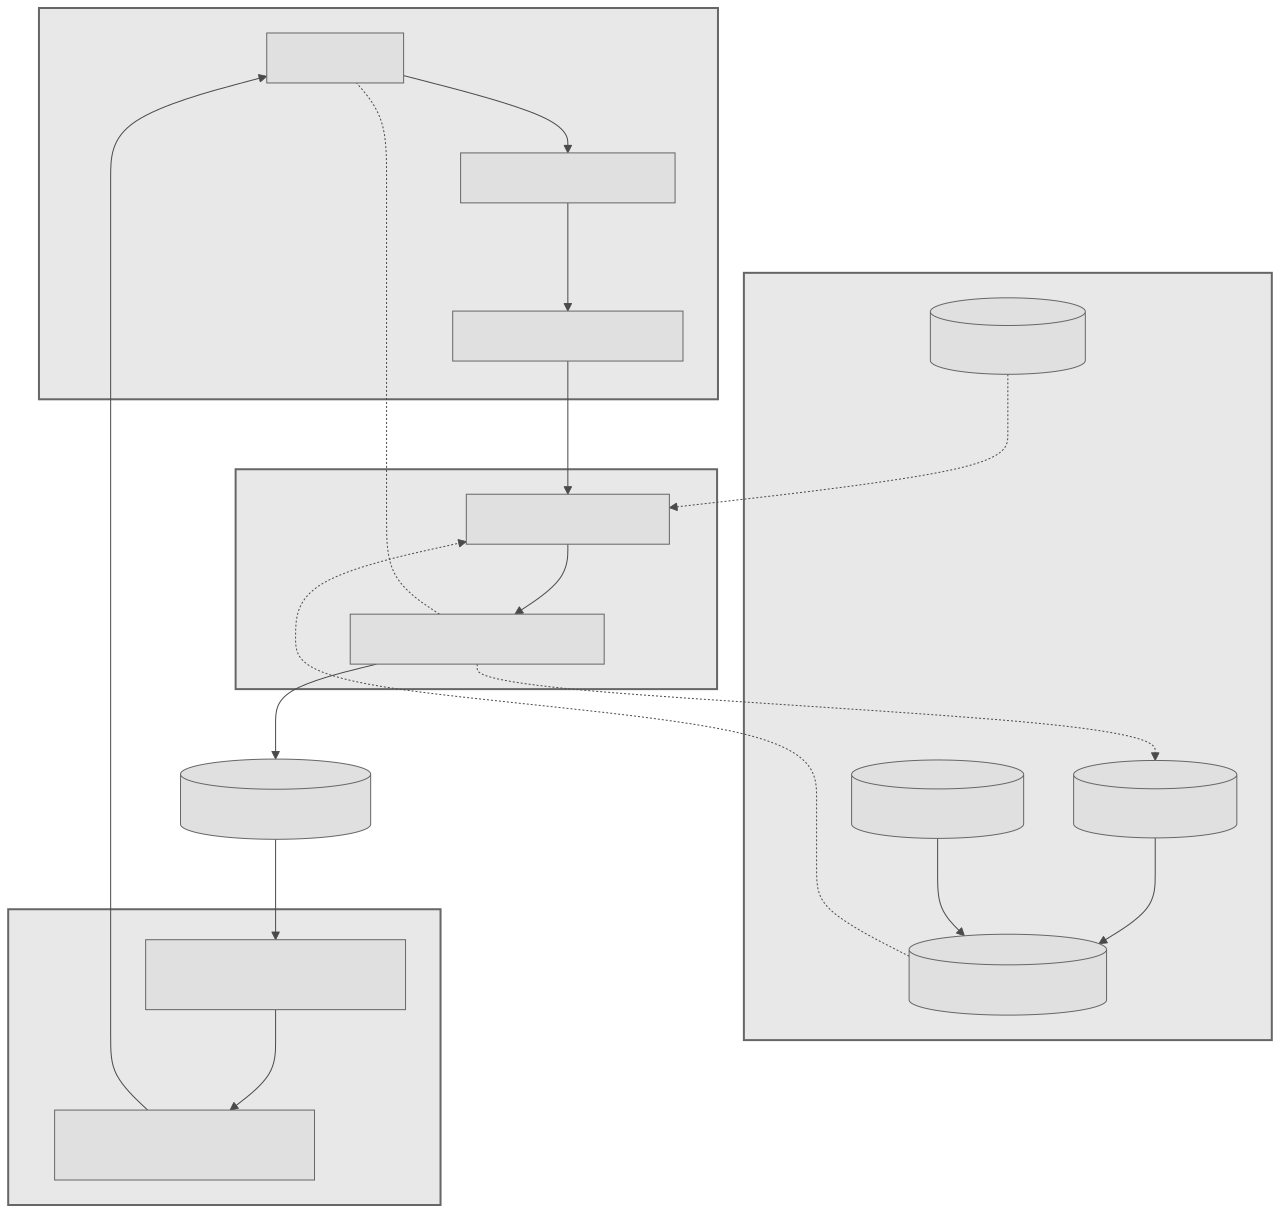
\includegraphics[width=0.95\textwidth,keepaspectratio]{figures/architecture.mmd.png}
\caption{Healthcare Analytics Architecture. Solid lines indicate the primary data flow from clinical user natural language queries through a conversational AI interface to a healthcare NLP engine for context-aware SQL generation. Bi-directional arrows at steps 5 and 8 represent the iterative 'Query \& Refine' loop where users refine their intent based on delivered insights. The critical validation step (dotted bi-directional line) shows domain experts confirming or correcting generated SQL before results are trusted. Validated NL+SQL pairs flow to organizational memory (dashed line), where they persist independent of staff tenure and inform future query generation.}
\label{fig:architecture}
\end{figure}

\subsubsection{Illustrative Application: The Validated Query Cycle as a
Governance Forcing
Function}\label{illustrative-application-the-validated-query-cycle-as-a-governance-forcing-function}

To demonstrate how the three-pillar framework might inform technology
design, we describe a validated query cycle. This cycle functions as a
\textbf{Governance Forcing Function}, a mechanism that uses technical
implementation to compel the adoption of stronger data governance
practices. It directly addresses institutional memory loss (Pillar 2) by
systematically converting tacit knowledge into an explicit, durable
asset, thereby reducing technical barriers (Pillar 3) and enabling
organizations to advance their analytics maturity (Pillar 1).

The six-step cycle (Figure 2) illustrates this approach:

\begin{enumerate}
\def\labelenumi{\arabic{enumi}.}
\item
  \textbf{Query}: A domain expert (clinician, analyst, or administrator)
  asks a natural language question, such as, ``What was our 30-day
  readmission rate for heart failure patients last quarter?''
\item
  \textbf{Generation}: The conversational AI system generates candidate
  SQL code, leveraging healthcare ontologies and organizational schema
  knowledge.
\item
  \textbf{Validation}: The AI provides a natural language explanation of
  the SQL logic and results, allowing the domain expert to validate the
  query's intent without reviewing raw code. This human-in-the-loop step
  aligns with ``Human-on-the-Loop'' (HotL) frameworks, transforming
  validation from a binary check into an iterative knowledge capture
  process
  (\citeproc{ref-bravorocca2023}{\textbf{bravorocca2023?}},\citeproc{ref-mosqueirarey2023}{\textbf{mosqueirarey2023?}}).
  This is essential given that current models are ``not yet sufficiently
  accurate for unsupervised use'' in clinical settings
  (\citeproc{ref-ziletti2024}{\textbf{ziletti2024?}}).
\item
  \textbf{Storage}: Once validated, the NL+SQL pair is stored in
  organizational memory as a durable knowledge artifact, along with
  mandatory ``Rationale Metadata'' documenting the query's business
  logic (e.g., ``Excluding Hospice per 2025 CMS rules'').
\item
  \textbf{Retrieval}: When future users ask similar questions, the
  system retrieves relevant validated pairs, reducing dependence on
  individual expertise.
\item
  \textbf{Persistence}: When the original expert leaves, their
  analytical knowledge remains embedded in the system. New staff inherit
  executable knowledge rather than starting from scratch.
\end{enumerate}

\begin{figure}[htbp]
\centering
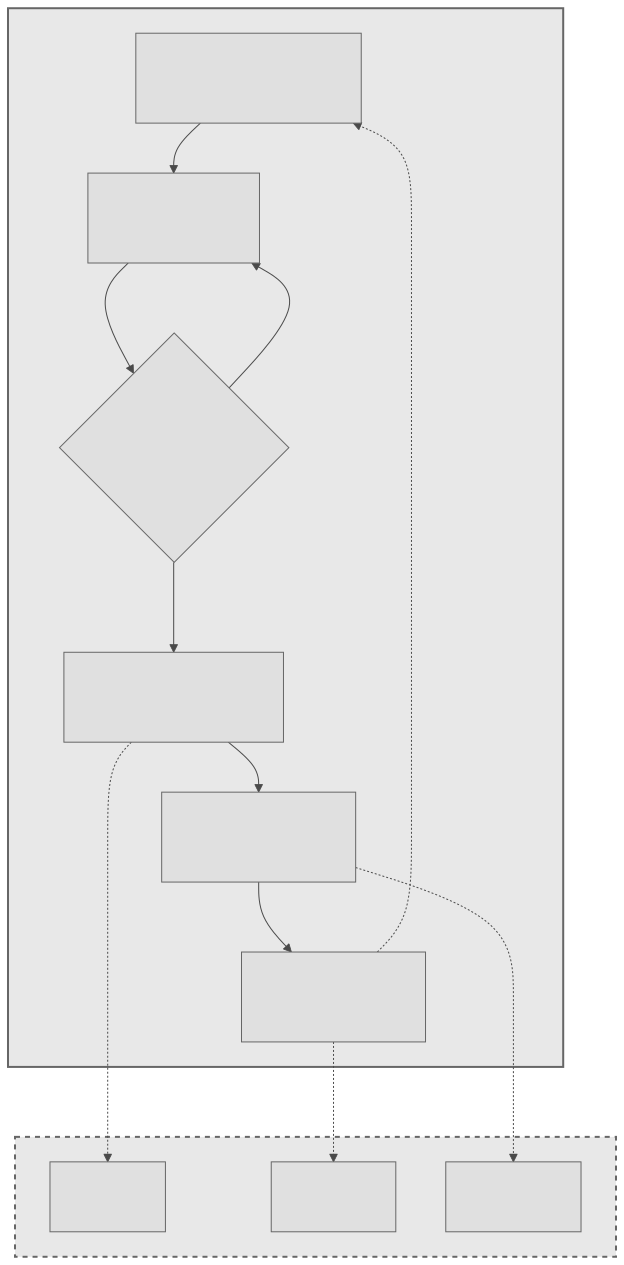
\includegraphics[width=0.5\textwidth,keepaspectratio]{figures/knowledge-cycle.mmd.png}
\caption{The Validated Query Cycle, shown as six numbered steps in the diagram. (1) Domain experts ask natural language questions, (2) the system generates candidate SQL, (3) AI provides a natural language explanation of the SQL logic; domain expert confirms the intent and results, (4) validated pairs are stored, (5) future queries retrieve validated knowledge, and (6) expertise persists through staff turnover. This cycle breaks the compounding effect where turnover erases institutional memory.}
\label{fig:knowledge-cycle}
\end{figure}

This cycle breaks the compounding effect identified in the three-pillar
framework: turnover no longer erases analytical knowledge because
expertise is embedded in validated query pairs rather than individual
memory. Low-maturity organizations can accelerate advancement by
accumulating validated queries, and technical barriers are reduced
because new staff access proven query patterns rather than recreating
analytical logic.

\subsection{Document Structure}\label{document-structure}

Following this introduction, the paper proceeds through five main
sections. The Methodology section describes the narrative review
approach, literature search strategy, and source selection criteria. The
Framework Development section documents how the three-pillar framework
emerged from the literature and its theoretical grounding. The
Literature Review synthesizes evidence across the three pillar domains:
natural language to SQL generation, analytics maturity, and workforce
dynamics. The Discussion examines implications, limitations, and future
research directions. Finally, the Conclusion summarizes the three-pillar
analytical framework as this paper's primary contribution to healthcare
informatics literature.

\section{Methodology}\label{methodology}

\subsection{Review Approach}\label{review-approach}

This paper employs a narrative review methodology to synthesize evidence
across the three pillars of the framework: analytics maturity, workforce
agility, and technical enablement (specifically natural language to SQL
generation). Unlike systematic reviews that follow pre-registered
protocols with exhaustive searches, narrative reviews provide expert
synthesis of relevant literature to construct coherent arguments and
identify patterns across diverse evidence sources.

The narrative review approach was selected because:

\begin{enumerate}
\def\labelenumi{\arabic{enumi}.}
\tightlist
\item
  \textbf{Integration across domains}: The paper synthesizes evidence
  from distinct fields (clinical informatics, human resources, natural
  language processing) that require interpretive integration rather than
  statistical pooling
\item
  \textbf{Original analytical framework}: The three-pillar framework
  emerged iteratively from the literature rather than being
  pre-specified
\item
  \textbf{Heterogeneous evidence types}: The evidence base includes
  peer-reviewed research, industry reports, and benchmark datasets that
  cannot be meaningfully combined through meta-analysis
\end{enumerate}

\subsection{Stage 1: Identification and Targeted
Queries}\label{stage-1-identification-and-targeted-queries}

Literature was identified through multiple channels between January 2023
and December 2025:

\textbf{Academic Databases:}

\begin{itemize}
\tightlist
\item
  Crossref: Cross-disciplinary academic literature, citation metadata
\item
  PubMed: Clinical informatics, healthcare workforce, medical
  administration
\item
  arXiv: Machine learning and NLP preprints, benchmark studies
\item
  Semantic Scholar: AI and computer science papers, citation analysis
\end{itemize}

\textbf{Industry Sources:}

\begin{itemize}
\tightlist
\item
  HIMSS: Analytics Maturity Model documentation and industry standards
\item
  Healthcare providers: NHS Trust implementation case studies
\item
  Market research: Precedence Research, Forrester analyst reports
\item
  Technology vendors: Health Catalyst, Oracle, Anthropic technical
  documentation
\item
  Professional associations: AHIMA/NORC workforce surveys
\item
  Business news: IBM, CNBC coverage of healthcare analytics ventures
\end{itemize}

\textbf{Search Concepts and Results:}

Search terms emerged iteratively and were organized around the
three-pillar framework. Table 1 summarizes the search concepts and
results by source.

\begin{longtable}[]{@{}lccccc@{}}
\caption{Initial search results by database source. Numbers in
parentheses indicate studies passing initial screening. Search concepts:
\textbf{Analytics Maturity} (``healthcare analytics maturity'', ``HIMSS
AMAM'', ``analytics adoption'', ``big data analytics adoption'',
``resistance to change'', ``analytics standardization failure'',
``low-code ROI''); \textbf{Workforce Agility} (``healthcare IT tenure'',
``IT training time'', ``turnover cost'', ``institutional memory loss'',
``organizational forgetting'', ``competence loss'', ``knowledge
portal'', ``SECI model''); \textbf{Technical Enablement} (``NL2SQL
healthcare'', ``text-to-SQL clinical'', ``MIMICSQL'', ``EHRSQL'',
``schema discovery'', ``semantic column matching'', ``vector
embeddings'').}\tabularnewline
\toprule\noalign{}
Pillar & Crossref & PubMed & arXiv & Sem. Scholar & Total (Screened) \\
\midrule\noalign{}
\endfirsthead
\toprule\noalign{}
Pillar & Crossref & PubMed & arXiv & Sem. Scholar & Total (Screened) \\
\midrule\noalign{}
\endhead
\bottomrule\noalign{}
\endlastfoot
\textbf{Analytics Maturity} & 285 & - & - & - & 285 (15) \\
\textbf{Workforce Agility} & - & 142 & - & - & 142 (12) \\
\textbf{Technical Enablement} & - & - & 71 & 72 & 143 (14) \\
\textbf{Total} & \textbf{285} & \textbf{142} & \textbf{71} & \textbf{72}
& \textbf{570 (41)} \\
\end{longtable}

The final corpus includes 115 academic and 20 industry sources (135
total). Targeted queries were employed to address specific evidence gaps
identified during the synthesis process.

Figure 3 illustrates the literature selection process, showing
progression from initial database search through screening and quality
assessment to the final corpus of included sources.

\begin{figure}[htbp]
\centering
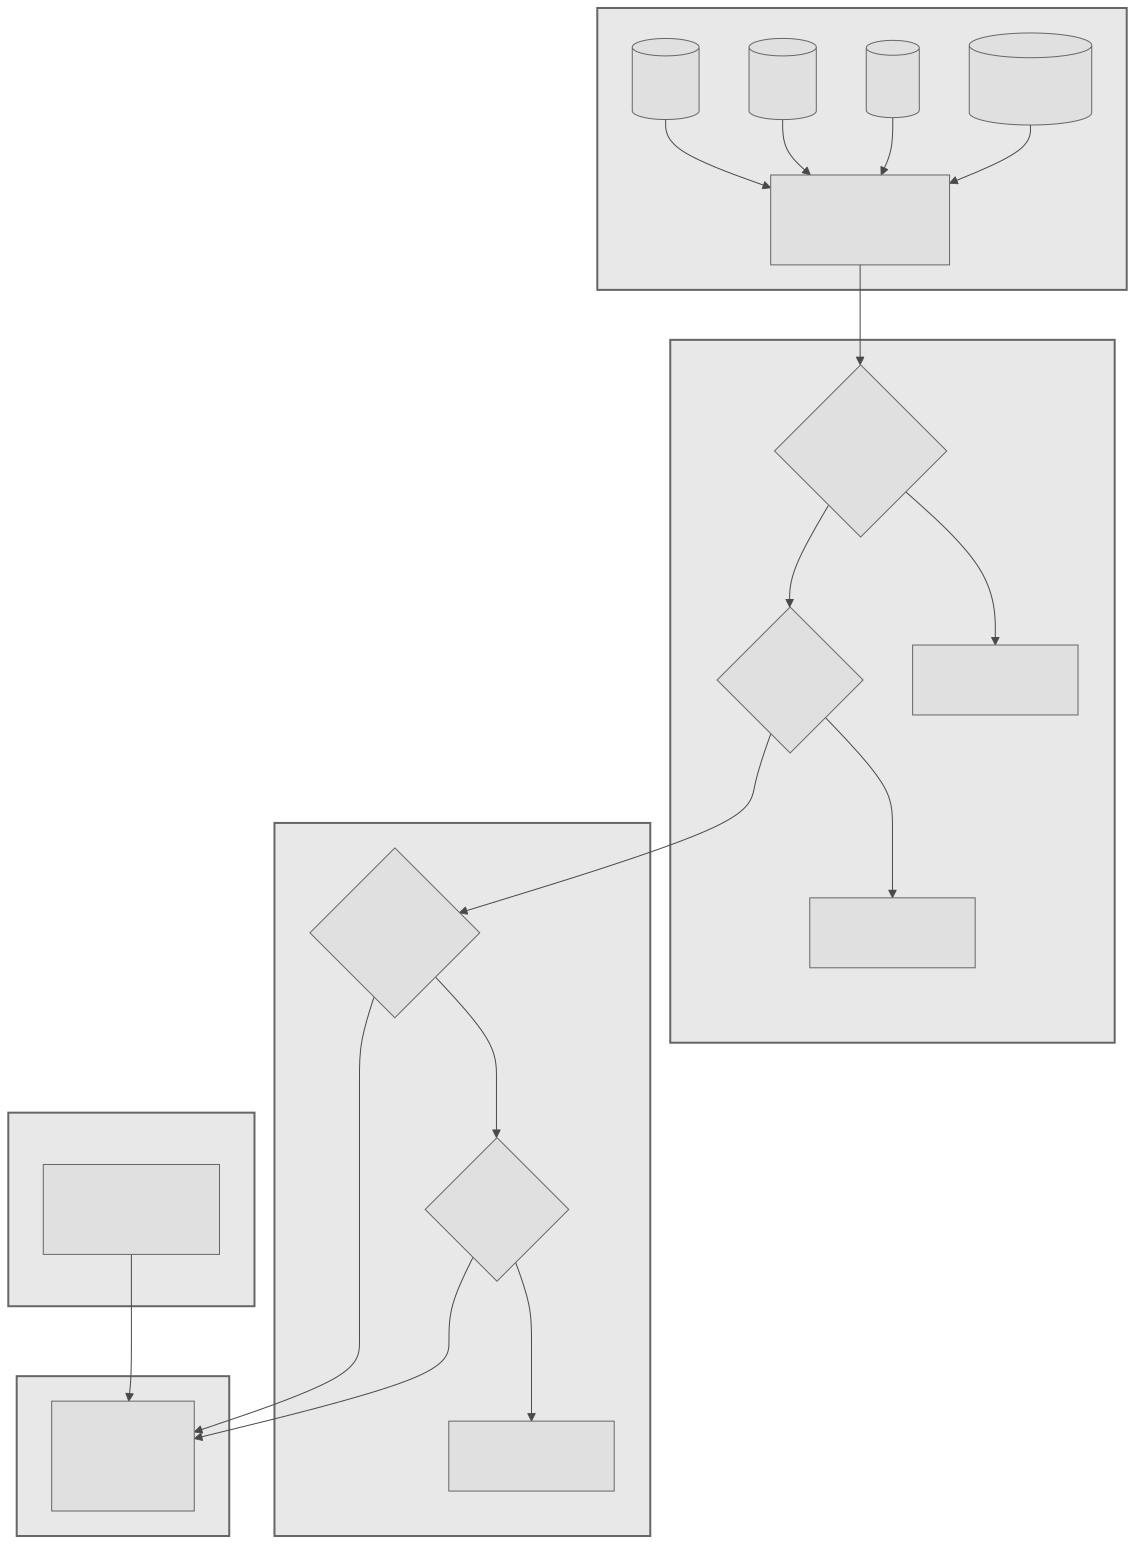
\includegraphics[width=0.9\textwidth,keepaspectratio]{figures/literature-flow.mmd.png}
\caption{Literature Selection Flow Diagram. The diagram shows the progression from initial database search (n ≈ 570) through title/abstract screening, full-text review, and quality assessment (AACODS for grey literature) to the final corpus of 135 sources (115 academic, 20 industry). Diagram source available in figures/literature-flow.mmd.}
\label{fig:literature-flow}
\end{figure}

\subsection{Stage 2: Screening and
Selection}\label{stage-2-screening-and-selection}

Sources were selected based on the following criteria:

\textbf{Inclusion Criteria:}

\begin{itemize}
\tightlist
\item
  Peer-reviewed publications in healthcare informatics, medical
  informatics, computer science, or health services research
\item
  Industry reports from established healthcare IT organizations (HIMSS,
  AHIMA, AMIA)
\item
  Publications from 2015-current, with emphasis on 2020-current for
  rapidly evolving NL2SQL technologies
\item
  English language publications
\item
  Sources with verifiable DOIs, URLs, or institutional attribution
\end{itemize}

\textbf{Exclusion Criteria:}

\begin{itemize}
\tightlist
\item
  Sources without verifiable attribution or institutional backing
\item
  Vendor marketing materials without independent validation
\item
  Preprints without subsequent peer-reviewed publication (exception:
  foundational NL2SQL benchmarks where peer review is pending)
\item
  Studies with unverifiable statistics or methodological concerns
\end{itemize}

\subsection{Stage 3: Quality
Assessment}\label{stage-3-quality-assessment}

Grey literature sources were assessed using the AACODS checklist
(\citeproc{ref-tyndall2010}{\textbf{tyndall2010?}}), which evaluates
Authority, Accuracy, Coverage, Objectivity, Date, and Significance.
Sources with vendor sponsorship were retained when no independent
alternative existed but flagged in-text. Table 2 summarizes the
assessment.

\begin{longtable}[]{@{}
  >{\raggedright\arraybackslash}p{(\columnwidth - 10\tabcolsep) * \real{0.3200}}
  >{\raggedright\arraybackslash}p{(\columnwidth - 10\tabcolsep) * \real{0.2080}}
  >{\raggedright\arraybackslash}p{(\columnwidth - 10\tabcolsep) * \real{0.1920}}
  >{\raggedright\arraybackslash}p{(\columnwidth - 10\tabcolsep) * \real{0.1600}}
  >{\raggedright\arraybackslash}p{(\columnwidth - 10\tabcolsep) * \real{0.0800}}
  >{\raggedright\arraybackslash}p{(\columnwidth - 10\tabcolsep) * \real{0.0080}}@{}}
\caption{AACODS Assessment of Industry Sources.
\label{tbl:aacods}}\tabularnewline
\toprule\noalign{}
\begin{minipage}[b]{\linewidth}\raggedright
Source (Citation)
\end{minipage} & \begin{minipage}[b]{\linewidth}\raggedright
Authority / Accuracy
\end{minipage} & \begin{minipage}[b]{\linewidth}\raggedright
Coverage / Objectivity
\end{minipage} &
\multicolumn{3}{>{\raggedright\arraybackslash}p{(\columnwidth - 10\tabcolsep) * \real{0.2480} + 4\tabcolsep}@{}}{%
\begin{minipage}[b]{\linewidth}\raggedright
Date / Significance\textbar{} Include
\end{minipage}} \\
\midrule\noalign{}
\endfirsthead
\toprule\noalign{}
\begin{minipage}[b]{\linewidth}\raggedright
Source (Citation)
\end{minipage} & \begin{minipage}[b]{\linewidth}\raggedright
Authority / Accuracy
\end{minipage} & \begin{minipage}[b]{\linewidth}\raggedright
Coverage / Objectivity
\end{minipage} &
\multicolumn{3}{>{\raggedright\arraybackslash}p{(\columnwidth - 10\tabcolsep) * \real{0.2480} + 4\tabcolsep}@{}}{%
\begin{minipage}[b]{\linewidth}\raggedright
Date / Significance\textbar{} Include
\end{minipage}} \\
\midrule\noalign{}
\endhead
\bottomrule\noalign{}
\endlastfoot
HIMSS AMAM (\citeproc{ref-himss2024}{\textbf{himss2024?}}) & High† /
Verifiable & Global / High & 2024 / High & Yes & \\
Snowdon/HIMSS (\citeproc{ref-snowdon2024b}{\textbf{snowdon2024b?}}) &
High‡ / Verifiable & N/A / High & 2024 / Medium & Yes & \\
Health Catalyst (\citeproc{ref-health2020}{\textbf{health2020?}}) &
Medium§ / Unverifiable & US / Low & 2020 / Medium & Yes* & \\
Berkshire NHS (\citeproc{ref-berkshire2024}{\textbf{berkshire2024?}}) &
High¶ / Verifiable & Single site / High & 2024 / High & Yes & \\
Forrester/Microsoft
(\citeproc{ref-forrester2024}{\textbf{forrester2024?}}) & Medium∥ /
Unverifiable & Enterprise / Low♢ & 2024 / Medium & Yes* & \\
Oracle (\citeproc{ref-oracle2024}{\textbf{oracle2024?}}) & Low§ /
Unverifiable & N/A / Low & 2024 / Low & Yes* & \\
Precedence Research
(\citeproc{ref-precedence2024}{\textbf{precedence2024?}}) & Medium\# /
Unverifiable & Global / Medium & 2024 / Medium & Yes & \\
Anthropic (\citeproc{ref-anthropic2025}{\textbf{anthropic2025?}}) &
Medium§ / Verifiable & N/A / Medium & 2025 / Low & Yes & \\
IBM Newsroom (\citeproc{ref-ibm2022}{\textbf{ibm2022?}}) & High** /
Verifiable & N/A / High & 2022 / High & Yes & \\
CNBC/Haven (\citeproc{ref-lavito2021}{\textbf{lavito2021?}}) & High** /
Verifiable & N/A / High & 2021 / High & Yes & \\
AHIMA/NORC (\citeproc{ref-american2023}{\textbf{american2023?}}) &
High†† / Verifiable & US / High & 2023 / High & Yes & \\
\end{longtable}

†Industry standards body. ‡HIMSS officer. §Vendor. ¶NHS trust. ∥Analyst
firm. \#Market research. **Journalism. ††Professional association +
academic. ♢Sponsor. *Vendor sponsorship or low objectivity noted in
manuscript text.

\subsection{Stage 4: Synthesis and
Analysis}\label{stage-4-synthesis-and-analysis}

Reflecting the framework's iterative emergence from the literature,
evidence is synthesized thematically below:

\begin{enumerate}
\def\labelenumi{\arabic{enumi}.}
\tightlist
\item
  \textbf{Analytics maturity}: Evidence on HIMSS AMAM adoption,
  healthcare analytics capabilities, and organizational readiness
\item
  \textbf{Workforce turnover}: Evidence on nursing and IT staff turnover
  rates, institutional memory loss, and knowledge transfer challenges
\item
  \textbf{Technical barriers}: Evidence on NL2SQL benchmarks,
  healthcare-specific NLP challenges, and low-code implementation
  patterns
\end{enumerate}

This framework emerged iteratively from the literature rather than being
pre-specified, consistent with narrative review methodology.

\subsection{Methodological
Limitations}\label{methodological-limitations}

This narrative review has inherent limitations:

\begin{itemize}
\tightlist
\item
  \textbf{Non-exhaustive search}: Literature identification was
  selective rather than exhaustive; relevant studies may have been
  missed
\item
  \textbf{Limited formal quality assessment}: Grey literature sources
  were assessed using the AACODS checklist; however, no standardized
  quality assessment tool (e.g., GRADE, Cochrane Risk of Bias) was
  applied to peer-reviewed sources, as these tools are designed for
  clinical intervention studies rather than narrative reviews
\item
  \textbf{Single-coder bias risk}: Literature screening, data
  extraction, and thematic analysis were performed by a single author
  without independent verification. This introduces potential selection
  and interpretation bias that would be mitigated in systematic reviews
  through dual-coder protocols with inter-rater reliability assessment
\item
  \textbf{Post-hoc selection criteria}: Inclusion and exclusion criteria
  were refined during the review process rather than pre-registered
\item
  \textbf{No protocol registration}: This review was not registered in
  PROSPERO or similar registries
\item
  \textbf{Dated workforce statistics}: The primary healthcare IT
  turnover statistic (\textasciitilde34\% implied for new hires) derives
  from Ang and Slaughter's 2004 study
  (\citeproc{ref-ang2004}{\textbf{ang2004?}}). While recent surveys
  confirm workforce challenges persist
  (\citeproc{ref-american2023}{\textbf{american2023?}}) and contemporary
  evidence suggests the situation may have worsened (55\% intent to
  leave among public health informatics specialists
  (\citeproc{ref-rajamani2025}{\textbf{rajamani2025?}})), no study has
  directly replicated the 2004 tenure measurement methodology. This
  paper reframes this ``data desert'' as evidence of the crisis itself:
  the industry is too unstable to track its own attrition effectively.
  Future research should address this methodological gap.
\end{itemize}

These limitations are balanced against the strengths of narrative review
methodology: ability to synthesize heterogeneous evidence types across
disciplinary boundaries, flexibility to pursue emerging themes, and
capacity to construct novel analytical frameworks that illuminate
connections between previously disconnected research domains.

\section{Framework Development and
Validation}\label{framework-development-and-validation}

This paper's primary contribution is the three-pillar analytical
framework for understanding healthcare analytics challenges: (1)
analytics maturity, (2) workforce agility, and (3) technical enablement.
This section documents the framework's development process and
theoretical grounding.

\subsection{Framework Development
Process}\label{framework-development-process}

The three-pillar framework emerged through iterative analysis of the
literature corpus. Initial review identified numerous disconnected
research streams: NL2SQL technical advances, HIMSS maturity models,
healthcare workforce turnover studies, knowledge management theory, and
healthcare IT implementation case studies. These appeared as isolated
topics until thematic analysis revealed recurring patterns of
interdependence.

The framework development followed these steps:

\begin{enumerate}
\def\labelenumi{\arabic{enumi}.}
\tightlist
\item
  \textbf{Theme Extraction}: Systematic coding of included sources
  identified recurring themes across technical, organizational, and
  workforce dimensions
\item
  \textbf{Pattern Recognition}: Cross-domain analysis revealed that
  challenges in each dimension amplified challenges in others. A root
  cause analysis (observation-why-repeat) determined the framework's
  ordering: low \textbf{Analytics Maturity} (Observation/Context) is
  driven by low \textbf{Workforce Agility} (Cause/Actor), which in turn
  is exacerbated by low \textbf{Technical Enablement} (Root
  Mechanism/Tool). This causal chain frames the three pillars, drawing
  on established RCA methodology for organizational learning
  (\citeproc{ref-allison2021}{\textbf{allison2021?}},\citeproc{ref-soylemez2017}{\textbf{soylemez2017?}}).
\item
  \textbf{Pillar Identification}: Three orthogonal yet interconnected
  dimensions emerged as the organizing structure:

  \begin{itemize}
  \tightlist
  \item
    \textbf{Analytics Maturity}: Organizational capability progression
    measured against HIMSS AMAM stages
  \item
    \textbf{Workforce Agility}: Human capital retention and tacit
    knowledge preservation
  \item
    \textbf{Technical Enablement}: NL2SQL capabilities and
    healthcare-specific implementation solutions
  \end{itemize}
\item
  \textbf{Framework Validation}: Pillar structure tested against the
  full corpus to confirm comprehensive coverage without significant gaps
\end{enumerate}

\subsection{Theoretical Grounding}\label{theoretical-grounding}

The three-pillar framework aligns with established models in healthcare
informatics and knowledge management:

\begin{table}[htbp]
\centering
\begin{tabular}{p{3cm}p{3.5cm}p{3.5cm}p{3.5cm}}
\toprule
\textbf{Three \newline Pillars} & \textbf{HIMSS AMAM Alignment} & \textbf{DIKW \newline Hierarchy} & \textbf{Knowledge Management} \\
\midrule
Analytics \newline Maturity & Stages 0-7 \newline Progression & Data \newline → Information & Organizational learning \\
Workforce \newline Agility & Implicit in \newline Advanced Stages & Knowledge (tacit) \newline → Wisdom & Tacit knowledge transfer \\
Technical \newline Enablement & Stage 6-7 \newline Requirements & Information \newline → Knowledge & Knowledge \newline Codification \\
\bottomrule
\end{tabular}
\caption{Framework Alignment with Established Models}
\label{tab:framework-alignment}
\end{table}

The HIMSS Analytics Maturity Assessment Model
(\citeproc{ref-himss2024}{\textbf{himss2024?}}) provides organizational
benchmarks but does not explicitly address workforce knowledge
retention. The Data-Information-Knowledge-Wisdom (DIKW) hierarchy
(\citeproc{ref-rowley2007}{\textbf{rowley2007?}}) explains the
progression from raw data to actionable insight, but standard
formulations do not address institutional memory loss. The three-pillar
framework synthesizes these perspectives, positioning workforce dynamics
as the critical enabler connecting data access (analytics maturity) with
organizational wisdom (knowledge preservation). It draws on established
knowledge management theory for organizational learning
(\citeproc{ref-rao2006}{\textbf{rao2006?}},\citeproc{ref-massingham2018}{\textbf{massingham2018?}}),
tacit knowledge transfer
(\citeproc{ref-farnese2019}{\textbf{farnese2019?}},\citeproc{ref-foos2006}{\textbf{foos2006?}}),
and knowledge codification
(\citeproc{ref-benbya2004}{\textbf{benbya2004?}},\citeproc{ref-zhang2025}{\textbf{zhang2025?}})
to explain these connections.

\subsection{Framework Scope and
Limitations}\label{framework-scope-and-limitations}

The framework is descriptive rather than prescriptive; it provides an
analytical lens for understanding healthcare analytics challenges but
does not mandate specific solutions. Future research should empirically
validate pillar interdependencies through longitudinal organizational
studies and develop quantitative metrics for framework dimensions.

\section{Literature Review: Evidence Across the Three
Pillars}\label{literature-review-evidence-across-the-three-pillars}

This narrative review synthesizes evidence across the three pillar
domains: analytics maturity, workforce agility, and technical enablement
(specifically natural language to SQL generation). Drawing from
peer-reviewed research, industry reports, and benchmark datasets
identified through the methodology described in Section 2 (Methodology),
we document the current state of each pillar and reveal
interconnections. Analysis reveals three critical findings: (1)
healthcare analytics maturity remains low with most organizations
struggling at basic stages, (2) healthcare workforce turnover creates
institutional memory loss that traditional approaches fail to address,
and (3) natural language to SQL generation has evolved significantly but
faces healthcare-specific challenges requiring specialized solutions.
Evidence across these three domains reveals significant interconnections
and compounding effects that the three-pillar framework synthesizes.

\subsection{State of Healthcare Analytics
Maturity}\label{state-of-healthcare-analytics-maturity}

\subsubsection{Low Organizational
Maturity}\label{low-organizational-maturity}

The Healthcare Information Management Systems Society (HIMSS) Analytics
Maturity Assessment Model (AMAM) provides the industry standard for
measuring analytics capabilities. Recent data reveals a concerning state
of analytics maturity in healthcare organizations globally
(\citeproc{ref-himss2024}{\textbf{himss2024?}}). The newly revised
AMAM24 model, launched in October 2024, represents a significant
evolution from the original framework.

Snowdon (\citeproc{ref-snowdon2024b}{\textbf{snowdon2024b?}}), Chief
Scientific Research Officer at HIMSS, emphasizes that ``analytics as a
discipline has changed dramatically in the last five to 10 years,'' yet
healthcare organizations struggle to keep pace
(\citeproc{ref-wang2018}{\textbf{wang2018?}}). Research confirms
healthcare's adoption of analytics often lags behind other sectors such
as retail and banking, partly due to the complexity of implementing new
technology in clinical environments
(\citeproc{ref-wang2018}{\textbf{wang2018?}}),
(\citeproc{ref-wang2017}{\textbf{wang2017?}}). The newly revised AMAM
model shifts focus from technical capabilities to outcomes and AI
governance, requiring evidence of responsible algorithm monitoring
(\citeproc{ref-himss2024apac}{\textbf{himss2024apac?}}). This shift
drove the early 2025 validations of Tampa General Hospital and China
Medical University Hospital (CMUH) at Stage 7, confirming that AI
readiness is the new gatekeeper for analytics maturity
(\citeproc{ref-tgh2025}{\textbf{tgh2025?}},\citeproc{ref-cmuh2025}{\textbf{cmuh2025?}}).
Regional adoption dynamics reveal distinct structural drivers: while
North American adoption is largely market-driven by value-based care,
Middle Eastern adoption is often characterized by government-mandated
visions, such as Saudi Arabia's centralized push for digital health
excellence which has propelled institutions like King Faisal Specialist
Hospital to Stage 7 (\citeproc{ref-ksa2024}{\textbf{ksa2024?}}).

Quantitative evidence links organizational maturity to patient outcomes
through two related pathways. First, EMR adoption maturity provides
foundational infrastructure: cross-sectional studies using the HIMSS
Electronic Medical Record Adoption Model (EMRAM) demonstrate that
hospitals with advanced EMR adoption (levels 6-7) have 3.25 times higher
odds of achieving better Leapfrog Group Hospital Safety Grades compared
to hospitals at EMRAM level 0, with significantly reduced infection
rates and fewer adverse events
(\citeproc{ref-snowdon2024}{\textbf{snowdon2024?}}). Similarly,
high-maturity hospitals have 1.8 to 2.24 times higher odds of achieving
higher patient experience ratings
(\citeproc{ref-snowdon2024a}{\textbf{snowdon2024a?}}). Second, analytics
capabilities build on this digital foundation: big data analytics
capabilities, combined with complementary organizational resources and
analytical personnel skills, improve readmission rates and patient
satisfaction (\citeproc{ref-wang2019}{\textbf{wang2019?}}), while
poor-quality data results in diagnostic errors, ineffective treatments,
and compromised patient care
(\citeproc{ref-gomes2025}{\textbf{gomes2025?}}). Note that EMRAM
measures EMR adoption stages rather than analytics maturity directly;
robust digital infrastructure is a prerequisite for analytics, but the
AMAM model addresses the analytics-specific capability gap. However,
evidence explicitly linking the new AMAM framework to outcomes remains
sparse. Studies relying on older proxies yield mixed results: while some
align digital maturity with lower staff turnover and reduced errors
(\citeproc{ref-woods2024}{\textbf{woods2024?}}), others find no
significant association with readmission rates
(\citeproc{ref-saintulysse2021}{\textbf{saintulysse2021?}}) or mortality
(\citeproc{ref-martin2019}{\textbf{martin2019?}}), suggesting that
maturity alone is insufficient without workforce stability.

\subsubsection{Barriers to Analytics
Adoption}\label{barriers-to-analytics-adoption}

A systematic literature review of big data analytics in healthcare by
Kamble et al. (\citeproc{ref-kamble2019}{\textbf{kamble2019?}})
identifies critical barriers to analytics adoption. The study reveals
that healthcare enterprises struggle with technology selection, resource
allocation, and organizational readiness for data-driven decision
making.

Health Catalyst's Healthcare Analytics Adoption Model
(\citeproc{ref-health2020}{\textbf{health2020?}}), a vendor-produced
framework, corroborates these findings, documenting that most healthcare
organizations remain at Stages 0-3, characterized by:

\begin{itemize}
\tightlist
\item
  Fragmented data sources without integration
\item
  Limited automated reporting capabilities
\item
  Lack of standardized data governance
\item
  Minimal predictive or prescriptive analytics
\item
  Absence of real-time decision support
\end{itemize}

\subsubsection{The Analytics Skills Gap}\label{the-analytics-skills-gap}

The literature consistently identifies workforce capabilities as a
primary constraint. Healthcare organizations face mounting challenges in
extracting meaningful insights from the vast amount of unstructured
clinical text data generated daily
(\citeproc{ref-navarro2023}{\textbf{navarro2023?}}). There is an
acknowledged problem in health services where organizations cannot make
good use of available data due to a deficit in skilled analysts across
all sectors and levels
(\citeproc{ref-bardsley2016}{\textbf{bardsley2016?}}). Organizations
face critical challenges in recruiting and retaining professionals with
the right analytical skills, while the need for big data specialists
with analytical capabilities continues to grow
(\citeproc{ref-pesqueira2020}{\textbf{pesqueira2020?}}). Traditional
approaches to analytics require extensive technical expertise and time
that healthcare professionals typically lack, creating a fundamental
barrier to analytics adoption
(\citeproc{ref-american2023}{\textbf{american2023?}}).

\subsubsection{Data Quality as a Barrier to Analytics
Maturity}\label{data-quality-as-a-barrier-to-analytics-maturity}

Beyond workforce constraints, data quality represents a fundamental
barrier preventing healthcare organizations from advancing their
analytics capabilities. Research consistently demonstrates that data
quality is both a prerequisite for and a dimension of analytics
maturity; organizations cannot progress to higher maturity stages
without first addressing data quality issues
(\citeproc{ref-carvalho2019}{\textbf{carvalho2019?}}). Multiple maturity
frameworks, including the Healthcare Data Quality Maturity Model (HDQM2)
and the Data Analytics Maturity Assessment Framework (DAMAF), explicitly
incorporate data quality as a core assessment dimension
(\citeproc{ref-pintovalverde2013}{\textbf{pintovalverde2013?}},\citeproc{ref-gokalp2023}{\textbf{gokalp2023?}}).
A cross-industry survey found that data management and quality issues,
including lack of documentation, accuracy, and consistency, continue to
challenge analytics organizations even as they mature, with the specific
challenges shifting from integration to privacy and documentation
concerns at higher maturity levels
(\citeproc{ref-lismont2017}{\textbf{lismont2017?}}).

The prevalence of data quality issues in healthcare databases is
substantial. A study of the National Cancer Database found missing data
rates ranging from 39.7\% for prostate cancer to 71.0\% for non-small
cell lung cancer (\citeproc{ref-yang2021}{\textbf{yang2021?}}). Medical
registry data shows 2.0\% to 4.6\% inaccurate records and 5\% to 6\%
incomplete data (\citeproc{ref-arts2002}{\textbf{arts2002?}}). Duplicate
patient records affect 0.16\% to 15.47\% of records across healthcare
institutions, with wide variation in management practices
(\citeproc{ref-mccoy2013}{\textbf{mccoy2013?}}). Analysis of Medicaid
claims data found that 9.74\% of data cells contained defects, with
issues frequently remaining obscure due to separation between data users
and producers (\citeproc{ref-zhang2024}{\textbf{zhang2024?}}).

Critically, automated data quality tools alone are insufficient for
healthcare data. Research demonstrates that clinical domain expert
involvement is necessary at every stage of the data pipeline, including
curation, cleaning, and analysis
(\citeproc{ref-rahman2020}{\textbf{rahman2020?}}). Automated tools fail
to detect context-dependent errors such as mutually exclusive values,
definitional differences between institutions, or plausibility issues
that require clinical judgment
(\citeproc{ref-sirgo2018}{\textbf{sirgo2018?}}). Even successful
automation requires embedding clinical knowledge; generic automated
cleaning tools from other domains are unsuitable for clinical data,
which requires variable-specific rules based on clinical knowledge of
normal ranges, extreme values, and clinical contexts
(\citeproc{ref-shi2021}{\textbf{shi2021?}}).

Compounding these challenges, healthcare database schemas are frequently
undocumented or poorly documented. Commercial EMR systems use
proprietary data models that are not publicly available, requiring
``detective work'' and reverse-engineering for research data integration
(\citeproc{ref-dugas2016}{\textbf{dugas2016?}},\citeproc{ref-bokov2017}{\textbf{bokov2017?}}).
A systematic review found that metadata models are often too complicated
for healthcare professionals without specific IT skills, resulting in
rare usage and poorly maintained documentation
(\citeproc{ref-ulrich2022}{\textbf{ulrich2022?}}). Poor chart
documentation by healthcare providers propagates downstream to
administrative data quality issues
(\citeproc{ref-lucyk2017}{\textbf{lucyk2017?}}). Most critically,
documentation knowledge is lost with staff changes: decisions based on
poorly documented data represent significant costs and risks, with
explicit identification of ``loss of information with staff changes'' as
a key vulnerability (\citeproc{ref-hovenga2013}{\textbf{hovenga2013?}}).

This creates a compounding effect across the three pillars: low-maturity
organizations have worse data quality and documentation, which requires
domain expertise to address, but that expertise is lost through
workforce turnover, further degrading data quality and preventing
maturity advancement. This persistent state of low maturity is not a
static condition but is actively driven by underlying workforce
dynamics, which the next section will explore.

\subsection{Healthcare Workforce Turnover and Knowledge
Loss}\label{healthcare-workforce-turnover-and-knowledge-loss}

\subsubsection{Turnover Rates and Financial
Impact}\label{turnover-rates-and-financial-impact}

While clinical turnover is well-studied
(\citeproc{ref-wu2024}{\textbf{wu2024?}},\citeproc{ref-ren2024}{\textbf{ren2024?}}),
technical staff turnover is more directly relevant to analytics maturity
and carries equally severe operational and financial consequences. Hong
(2025) demonstrates that turnover in federal IT roles directly degrades
organizational memory, causing a `sliding back' of performance
capabilities (\citeproc{ref-hong2025}{\textbf{hong2025?}}). This is
compounded by persistent vacancies; AHIMA/NORC (2023) report that 66\%
of health information professionals face staffing shortages, creating
bottlenecks that delay critical analytics initiatives
(\citeproc{ref-american2023}{\textbf{american2023?}}).

The financial impact of this instability is substantial. Massingham
(2018) demonstrates that the total cost of knowledge loss in specialized
sectors can reach three times the annual salary budget for the departing
role (\citeproc{ref-massingham2018}{\textbf{massingham2018?}}). In
healthcare, vendor analysis from Oracle (2024) corroborates this
``knowledge worker premium,'' documenting that turnover costs for
informatics and innovation-focused roles range from 1.5 to 2.0 times
annual salary due to the extreme scarcity of specialized digital skills
(\citeproc{ref-oracle2024}{\textbf{oracle2024?}}). These figures align
with established benchmarks for leadership departures, where recruitment
and lost productivity costs can exceed \$500,000 per specialist
(\citeproc{ref-willardgrace2019}{\textbf{willardgrace2019?}}).

Technical and analytics staff face acute instability that extends beyond
general turnover baselines. While hospital-wide data establishes a high
churn environment, with 30\% of all new employees (clinical and
non-clinical) leaving within their first year
(\citeproc{ref-nsi2025}{\textbf{nsi2025?}}), the crisis in informatics
roles is even more severe. Recent industry assessments reveal shortages
at both leadership and operational levels. Strategically, 53\% of
healthcare CIOs have held their current role for less than three years
(\citeproc{ref-wittkieffer2024}{\textbf{wittkieffer2024?}}), creating
leadership vacuums that disrupt long-term analytics initiatives.
Operationally, this instability is compounded by persistent vacancies,
with 79\% of healthcare provider organizations reporting shortages in
``Information and Digital Health'' roles
(\citeproc{ref-himssworkforce2024}{\textbf{himssworkforce2024?}}). This
creates a ``revolving door'' for innovation-focused staff, significantly
impacting the continuity required for complex modernization. The 2023
AHIMA/NORC workforce survey found that 66\% of health information
professionals report persistent staffing shortages, with 83\% reporting
that unfilled roles increased or remained stagnant over the past year
(\citeproc{ref-american2023}{\textbf{american2023?}}).

The knowledge loss implications are substantial. Research documents
significant time-to-productivity requirements across healthcare IT
roles: basic EHR training requires 8 hours to 2 months for end-users,
while health information workforce development demands 18 months to 2
years for specialized roles
(\citeproc{ref-ledikwe2013}{\textbf{ledikwe2013?}}). International
Medical Informatics Association recommendations specify a minimum of 1
year (60 ECTS credits) for biomedical and health informatics specialists
(\citeproc{ref-mantas2010}{\textbf{mantas2010?}}), with personalized EHR
training programs requiring 6 months of blended instruction to achieve
meaningful competency improvements
(\citeproc{ref-musa2023}{\textbf{musa2023?}}). For IT developers and
specialists, research suggests up to 3 years are required to become
fully fluent in complex healthcare IT projects
(\citeproc{ref-konrad2022}{\textbf{konrad2022?}}). Given that average
tenures often fall below the three-year proficiency threshold---with
CIOs averaging less than three years and new technical hires just 2.9
years
(\citeproc{ref-wittkieffer2024}{\textbf{wittkieffer2024?}},\citeproc{ref-ang2004}{\textbf{ang2004?}})---many
healthcare IT professionals spend only a limited portion of their
employment at full productivity and, in the case of IT developers, are
likely to leave before reaching full fluency. This creates a perpetual
cycle where organizations lose experienced staff before fully recouping
their training investment.

The impact on organizational capability is well-documented through the
lens of ``organizational forgetting.'' Rao and Argote (2006) establish
that high turnover rates disrupt the collective knowledge structures
required for complex task performance, effectively causing organizations
to ``forget'' established best practices
(\citeproc{ref-rao2006}{\textbf{rao2006?}}). This phenomenon is
particularly acute in knowledge-intensive sectors; Massingham (2018)
demonstrates that the departure of experienced staff leads to a
measurable ``loss of competence'' that forces remaining teams to regress
to earlier learning stages
(\citeproc{ref-massingham2018}{\textbf{massingham2018?}}). In the
context of healthcare analytics, this manifests not as immediate
clinical errors, but as a systemic inability to maintain the data
quality and interpretive context required for reliable decision-making.

\subsubsection{Institutional Memory
Loss}\label{institutional-memory-loss}

The concept of institutional memory in healthcare has received
increasing attention. Institutional memory encompasses the collective
knowledge, experiences, and expertise that enables organizational
effectiveness. Healthcare organizations typically lack formal mechanisms
for knowledge preservation, relying instead on person-to-person transfer
that fails during rapid turnover. Cultural and regulatory obstacles for
data sharing further limit the ability of healthcare organizations to
achieve the full potential of their data assets
(\citeproc{ref-mayo2016}{\textbf{mayo2016?}}).

When experienced analysts, clinical informatics professionals, or
data-savvy clinicians leave, they take with them irreplaceable knowledge
about data definitions, business rules, analytical approaches, and
organizational context. Research on tacit knowledge transfer provides
strong evidence that this knowledge is inherently difficult to document
through traditional means. Empirical studies demonstrate that learning
related to tacit knowledge is often not captured in formal post-project
review reports (\citeproc{ref-goffin2011}{\textbf{goffin2011?}}), and
conventional mechanisms such as documents, blueprints, and procedures
fail because tacit knowledge is not easily codified
(\citeproc{ref-foos2006}{\textbf{foos2006?}}). Research across multiple
industries consistently shows that written reports and databases fail to
convey key learning from expert teams
(\citeproc{ref-goffin2010}{\textbf{goffin2010?}}), while experts often
lack the skills, motivation, or time to document their expertise, and
even when documentation is attempted, essential aspects are lost due to
lack of shared experience between experts and novices
(\citeproc{ref-rintala2006}{\textbf{rintala2006?}}).

\subsubsection{Inadequacy of Traditional
Approaches}\label{inadequacy-of-traditional-approaches}

The literature demonstrates that conventional knowledge management
approaches fail in healthcare contexts
(\citeproc{ref-mayo2016}{\textbf{mayo2016?}},\citeproc{ref-shahbaz2019}{\textbf{shahbaz2019?}}):

\begin{itemize}
\tightlist
\item
  Traditional knowledge transfer mechanisms show limited effectiveness
\item
  Organizations struggle to capture and maintain analytical expertise
\item
  Security concerns and employee resistance to change slow the pace of
  information system acceptance
  (\citeproc{ref-shahbaz2019}{\textbf{shahbaz2019?}})
\item
  Person-to-person knowledge transfer fails during rapid turnover cycles
\end{itemize}

The failure of these traditional methods to preserve institutional
memory highlights the need for systemic solutions that can capture and
codify expertise at scale. Technical enablement, particularly through
modern AI and natural language interfaces, offers a potential mechanism
to address this gap, as the next section will discuss.

\subsection{State of Natural Language to SQL
Generation}\label{state-of-natural-language-to-sql-generation}

\subsubsection{Evolution and Technical
Advances}\label{evolution-and-technical-advances}

Recent systematic reviews document the rapid evolution of natural
language to SQL (NL2SQL) technologies. Ziletti and D'Ambrosi
(\citeproc{ref-ziletti2024}{\textbf{ziletti2024?}}) demonstrate that
retrieval augmented generation (RAG) approaches significantly improve
query accuracy when applied to electronic health records (EHRs), though
they note that ``current language models are not yet sufficiently
accurate for unsupervised use'' in clinical settings. This assessment,
based on 2024 models, has been challenged by late-2025 benchmarks
showing GPT-5 exceeds physician baselines on standardized medical
reasoning tasks
(\citeproc{ref-wang2025}{\textbf{wang2025?}},\citeproc{ref-openai2025}{\textbf{openai2025?}}),
suggesting the reasoning capabilities necessary for complex cohort
definition are now available, though human oversight remains recommended
for safety. Their work on the DE-SynPUF dataset shows that integrating
medical coding steps into the text-to-SQL process improves performance
over simple prompting approaches.

Benchmarking studies from 2024-2025
(\citeproc{ref-medagentbench2024}{\textbf{medagentbench2024?}},\citeproc{ref-wu2024a}{\textbf{wu2024a?}})
examining LLM-based systems for healthcare identify unique challenges:
medical terminology, characterized by abbreviations, synonyms, and
context-dependent meanings, remains a barrier to accurate query
generation. While previous models (GPT-4, Claude 3.5) achieved
\textasciitilde64-70\% accuracy on complex tasks, late-2025 models
demonstrate substantial improvements. GPT-5 achieves over 80\% accuracy
on complex medical reasoning benchmarks
(\citeproc{ref-wang2025}{\textbf{wang2025?}}). Crucially for analytics,
on healthcare-specific NL2SQL tasks, GPT-5 achieves 64.6\% execution
accuracy on the MIMICSQL dataset
(\citeproc{ref-blaskovic2025}{\textbf{blaskovic2025?}}), while the
HealthBench benchmark shows hallucination rates of 0.7-1.0\%,
representing a 4-6x improvement over previous models
(\citeproc{ref-openai2025}{\textbf{openai2025?}}).

\subsubsection{Healthcare-Specific
Challenges}\label{healthcare-specific-challenges}

The literature consistently identifies domain-specific obstacles in
healthcare NL2SQL implementation. A systematic review of NLP in EHRs
(\citeproc{ref-navarro2023}{\textbf{navarro2023?}}) found that the lack
of annotated data, automated tools, and other challenges hinder the full
utilization of NLP for EHRs. The review, following PRISMA guidelines,
categorized healthcare NLP applications into seven areas, with
information extraction and clinical entity recognition proving most
challenging due to medical terminology complexity.

Wang et al. (\citeproc{ref-wang2020}{\textbf{wang2020?}}) demonstrate
that healthcare NL2SQL methods must move beyond the constraints of exact
or string-based matching to fully encompass the semantic complexities of
clinical terminology. This work emphasizes that general-purpose language
models fail to capture the nuanced relationships between medical
concepts, diagnoses codes (ICD), procedure codes (CPT), and medication
vocabularies (RxNorm).

\subsubsection{Promising Approaches and
Limitations}\label{promising-approaches-and-limitations}

Recent advances show promise in addressing these challenges. The
TREQS/MIMICSQL dataset development
(\citeproc{ref-wang2020}{\textbf{wang2020?}}) and EHRSQL benchmark
(\citeproc{ref-lee2023}{\textbf{lee2023?}}) provide question-SQL pairs
specifically for healthcare, featuring questions in natural, free-form
language. Multi-modal benchmarks such as SM3-Text-to-Query
(\citeproc{ref-sivasubramaniam2024}{\textbf{sivasubramaniam2024?}})
extend evaluation beyond SQL to support multiple query languages across
diverse medical data representations. This approach acknowledges that
healthcare queries often require multiple logical steps: population
selection, temporal relationships, aggregation statistics, and
mathematical operations.

Healthcare-specific benchmarks continue to evolve alongside model
capabilities. The 2024 MedAgentBench evaluation found Claude 3.5 Sonnet
achieved 69.67\% success rate on medical agent tasks
(\citeproc{ref-medagentbench2024}{\textbf{medagentbench2024?}}),
(\citeproc{ref-wu2024a}{\textbf{wu2024a?}}); subsequent 2025 benchmarks
show GPT-5 significantly exceeding these results, with the SCARE
benchmark (\citeproc{ref-lee2025}{\textbf{lee2025?}}) providing 4,200
EHR question-SQL pairs across MIMIC-III, MIMIC-IV, and eICU databases
specifically designed to evaluate post-hoc safety mechanisms for
clinical text-to-SQL deployment. Graph-empowered approaches combining
LLMs with structured knowledge representations achieve 94.2\% execution
accuracy on MIMICSQL (\citeproc{ref-chen2025}{\textbf{chen2025?}}),
demonstrating that domain-specific architectural innovations can
substantially outperform general-purpose models. While these advances
narrow the gap between benchmark performance and clinical readiness,
domain-specific challenges in medical terminology and complex clinical
reasoning remain active research areas.

\subsubsection{Productivity and Efficiency
Evidence}\label{productivity-and-efficiency-evidence}

Emerging research documents quantifiable productivity gains from NL2SQL
implementations. In healthcare settings, organizations implementing
natural language interfaces report a 63\% increase in self-service
analytics adoption among non-technical staff and a 37\% reduction in
time spent on data retrieval tasks
(\citeproc{ref-dadi2025}{\textbf{dadi2025?}}). Business analysts using
these interfaces spend 42\% more time on analysis rather than query
construction (\citeproc{ref-dadi2025}{\textbf{dadi2025?}}).

Clinical-specific natural language interfaces demonstrate significant
efficiency improvements. Criteria2Query, a natural language interface
for clinical database cohort definition, achieves fully automated query
formulation in an average of 1.22 seconds per criterion, enabling
researchers to query EHR data without mastering database query languages
(\citeproc{ref-yuan2019}{\textbf{yuan2019?}}). The system has evolved
through three generations: the original rule-based approach
(\citeproc{ref-yuan2019}{\textbf{yuan2019?}}), a human-machine
collaboration version, and Criteria2Query 3.0, which leverages GPT-4 to
generate sharable cohort identification queries against OMOP-CDM
formatted databases (\citeproc{ref-park2024}{\textbf{park2024?}}). User
studies show NL2SQL systems reduce query completion times by 10-30\%
compared to traditional SQL platforms while improving accuracy from 50\%
to 75\%, with users recovering from errors 30-40 seconds faster
(\citeproc{ref-ipeirotis2025}{\textbf{ipeirotis2025?}}).

The most substantial productivity gains appear in multimodal interfaces.
Research on speech-driven database querying demonstrates users can
specify SQL queries with an average speedup of 2.7x (up to 6.7x)
compared to traditional input methods, with user effort reduced by a
factor of 10x to 60x compared to raw typing
(\citeproc{ref-shah2020}{\textbf{shah2020?}}). Healthcare-specific
natural language query systems show dramatic improvements: a clinical
data analytics language (CliniDAL) reduced complex query formulation
from ``many days'' with SQL to ``a few hours'' with natural language,
with expert users describing SQL as ``very tedious and time-consuming''
for the same analytical tasks
(\citeproc{ref-safari2014}{\textbf{safari2014?}}). NLP-driven data entry
systems have achieved 33\% time reduction with 15\% accuracy improvement
in clinical research settings
(\citeproc{ref-han2019}{\textbf{han2019?}}). Healthcare-specific NL2SQL
models such as MedT5SQL achieve 80.63\% exact match accuracy on the
MIMICSQL benchmark, demonstrating that domain-adapted language models
can effectively translate natural language to SQL for clinical databases
(\citeproc{ref-marshan2024}{\textbf{marshan2024?}}). These metrics
provide peer-reviewed evidence that complements vendor-sponsored
efficiency claims.

Code modernization principles directly inform these productivity gains.
Foundational work on natural language interfaces to databases
(\citeproc{ref-hendrix1978}{\textbf{hendrix1978?}}) established that
modular, decoupled architecture enables effective NL access to legacy
systems, a design principle applied across subsequent research (e.g.,
(\citeproc{ref-saha2023}{\textbf{saha2023?}})). Modern implementations
demonstrate that retrieval-augmented generation (RAG) approaches reduce
specialized training requirements by 87.4\% compared to traditional
querying methods while achieving 92.3\% accuracy in interpreting
business-specific terminology from legacy mainframe records
(\citeproc{ref-khandelwal2025}{\textbf{khandelwal2025?}}). This
convergence of code modernization and natural language interface
technologies arises because both rely on the same underlying large
language models (\citeproc{ref-ogunwole2023}{\textbf{ogunwole2023?}}),
(\citeproc{ref-arora2025}{\textbf{arora2025?}}), suggesting that
organizations investing in either capability simultaneously advance
both.

\subsection{Integration of Evidence: Synthesis Across Three
Pillars}\label{integration-of-evidence-synthesis-across-three-pillars}

\subsubsection{Pillar 1: Analytics Maturity and Democratized
Access}\label{pillar-1-analytics-maturity-and-democratized-access}

At its core, bridging technical and domain expertise serves a
fundamental patient care objective: enabling clinical professionals to
access and act on data that improves care quality. The convergence of
evidence reveals that traditional analytics maturity models often fail
because they assume a linear progression of \emph{technical} capability
rather than \emph{access} capability.

A critical distinction exists between traditional monitoring and dynamic
exploration. Visual dashboards excel at ``exploitation'' (monitoring
known metrics such as bed occupancy or infection rates) and provide
essential ``at-a-glance'' status
(\citeproc{ref-health2020}{\textbf{health2020?}}). However, dashboards
often create bottlenecks for novel or unanticipated clinical questions,
requiring a full build cycle and analyst intervention
(\citeproc{ref-syed2025}{\textbf{syed2025?}}). Conversational analytics
revolutionizes this ``time-to-insight'' by enabling ``exploration'' for
ad-hoc questions, reducing retrieval time from days to seconds
(\citeproc{ref-syed2025}{\textbf{syed2025?}}). Modern systems are
increasingly moving toward integrated ``Visual-Conversational''
interfaces, where natural language simplifies complex, nested queries
while visual panels align with clinical workflow needs for analytical
reasoning
(\citeproc{ref-samimi2025}{\textbf{samimi2025?}},\citeproc{ref-ruoff2023}{\textbf{ruoff2023?}}).
This integration facilitates a fluid, iterative exploration that
enhances both information-finding effectiveness and clinical
decision-making flow
(\citeproc{ref-chowdhury2020}{\textbf{chowdhury2020?}}). User studies
indicate that chatbot proficiency can be reached after a single task
repetition, suggesting a lower training burden for high-agility
enablement than traditional BI dashboards
(\citeproc{ref-holmes2019}{\textbf{holmes2019?}}). By democratizing
access, organizations can advance their effective maturity, the ability
to actually use data, even while backend infrastructure remains in
transition.

\subsubsection{Pillar 2: Workforce Agility and Institutional
Memory}\label{pillar-2-workforce-agility-and-institutional-memory}

The literature suggests that effective knowledge preservation requires
active, embedded systems rather than passive documentation
(\citeproc{ref-benbya2004}{\textbf{benbya2004?}},\citeproc{ref-whittaker2008}{\textbf{whittaker2008?}}).
The risk of institutional memory loss is not merely an HR issue but a
fundamental threat to analytics continuity
(\citeproc{ref-rao2006}{\textbf{rao2006?}}). When organizations choose
to implement AI-based platforms, these can serve as organizational
memory systems by:

\begin{itemize}
\tightlist
\item
  Capturing decision-making patterns through usage
  (\citeproc{ref-moore2018}{\textbf{moore2018?}})
\item
  Encoding best practices in accessible formats
  (\citeproc{ref-zhang2025}{\textbf{zhang2025?}})
\item
  Providing context-aware guidance to new users
\item
  Maintaining knowledge currency through continuous learning
\end{itemize}

These principles align with conversational AI approaches that embed
institutional knowledge within the AI model itself, making expertise
permanently accessible regardless of staff turnover
(\citeproc{ref-zhang2025}{\textbf{zhang2025?}}). This directly addresses
the Workforce Agility pillar by decoupling organizational capability
from individual tenure. When a senior analyst leaves, their ``validated
queries'' remain in the system, allowing a junior replacement to
immediately leverage that expertise rather than starting from zero,
mitigating the ``loss of competence'' effect described by Massingham
(2018) (\citeproc{ref-massingham2018}{\textbf{massingham2018?}}).

\subsubsection{Pillar 3: Technical Enablement as the
Catalyst}\label{pillar-3-technical-enablement-as-the-catalyst}

Technical enablement serves as the mechanism that breaks the compounding
cycle of low maturity and high turnover. Academic research provides
growing evidence for both conversational AI and low-code approaches as
effective catalysts in analytics workflows. In healthcare settings,
organizations implementing natural language interfaces report a 63\%
increase in self-service analytics adoption among non-technical staff
and a 37\% reduction in time spent on data retrieval tasks
(\citeproc{ref-dadi2025}{\textbf{dadi2025?}}). Precision medicine
platforms leveraging conversational AI have demonstrated 92.5\% accuracy
in parsing complex biomedical queries, executing tasks faster than
standard web portals (\citeproc{ref-yang2025}{1}). Furthermore,
experimental comparisons show that natural language interfaces can
accelerate database query formulation by 2.7x to 6.7x compared to
traditional methods (\citeproc{ref-shah2020}{\textbf{shah2020?}}),
reducing the dependency on specialized technical staff.

Low-code platforms and conversational AI represent complementary
approaches to this enablement
(\citeproc{ref-mogili2025}{\textbf{mogili2025?}}). Low-code platforms
provide visual development environments that accelerate application
development and reduce coding requirements, while conversational AI
enables natural language interaction with data systems. These approaches
share core benefits: both democratize access by enabling non-technical
users to perform complex analyses previously requiring data scientist
intervention (\citeproc{ref-berkshire2024}{\textbf{berkshire2024?}}),
both accelerate development cycles by abstracting technical complexity
(\citeproc{ref-aveiro2023}{\textbf{aveiro2023?}}), and both produce more
self-documenting systems where business logic is expressed in accessible
formats rather than specialized code. Evidence from low-code
implementations thus informs conversational AI adoption, as both address
the same fundamental barrier: the gap between clinical expertise and
technical capability.

Healthcare-specific studies show concrete benefits: Pennington
(\citeproc{ref-pennington2023}{\textbf{pennington2023?}}) found AI in
revenue cycle management accelerated payment cycles from 90 days to 40
days, while Atobatele et al.
(\citeproc{ref-atobatele2023}{\textbf{atobatele2023?}}) documented how
low-code platforms enable non-technical staff to build applications,
leading to efficiency gains. These findings collectively demonstrate
that technical enablement technologies produce measurable organizational
benefits not just by automating tasks, but by fundamentally changing
\emph{who} can perform them.

\subsection{Strategic Alignment with Industry
Trends}\label{strategic-alignment-with-industry-trends}

\subsubsection{Pillar 1 Alignment: Analytics Maturity
Trajectories}\label{pillar-1-alignment-analytics-maturity-trajectories}

Applied to recent industry literature, the three-pillar framework
highlights how barrier-reducing technologies track with broader
healthcare analytics trajectories. The revised HIMSS AMAM model
(\citeproc{ref-himss2024}{\textbf{himss2024?}}) emphasizes AI readiness
and governance frameworks, and conversational interfaces for analytics
can be understood as one illustrative application of these themes: they
aim to democratize access to data while preserving organizational
controls, rather than constituting a prescriptive pathway to maturity
advancement.

\subsubsection{Pillar 2 Alignment: Workforce Knowledge
Risks}\label{pillar-2-alignment-workforce-knowledge-risks}

The literature emphasizes that institutional memory loss represents an
existential risk to healthcare analytics programs, particularly when
critical analytical practices remain tacit and concentrated in a small
number of experts. Within our three-pillar framework, this risk appears
as a compounding mechanism: workforce turnover erodes tacit expertise,
low analytics maturity limits organizations' ability to encode that
expertise, and technical barriers constrain efforts to make encoded
knowledge broadly accessible. Effective knowledge preservation therefore
requires mechanisms that transform tacit analytical knowledge into
encoded, shareable, and routinely accessible artifacts. This requirement
aligns with Nonaka's SECI model (Socialization, Externalization,
Combination, Internalization), which describes organizational knowledge
creation as a continuous dialogue between tacit and explicit knowledge
(\citeproc{ref-farnese2019}{\textbf{farnese2019?}}). Recent research
demonstrates that AI tools, including conversational interfaces, can
enhance all four SECI stages, particularly facilitating the
externalization process where tacit analytical knowledge becomes
explicit, queryable forms
(\citeproc{ref-zhang2025}{\textbf{zhang2025?}}). This theoretical
foundation supports embedding organizational knowledge in systems rather
than individuals, ensuring continuity despite workforce turnover.

\subsubsection{Pillar 3 Alignment: Technical Enablement
ROI}\label{pillar-3-alignment-technical-enablement-roi}

Academic research documents multiple pathways to ROI for
barrier-reducing technologies in healthcare analytics. Conversational AI
implementations show direct benefits in analytical efficiency: Dadi et
al. (\citeproc{ref-dadi2025}{\textbf{dadi2025?}}) report a 63\% increase
in self-service analytics adoption among non-technical staff and a 37\%
reduction in data retrieval time. Precision medicine platforms have
demonstrated 92.5\% accuracy in parsing complex biomedical queries,
executing tasks significantly faster than standard web portals
(\citeproc{ref-yang2025}{1}). Furthermore, multimodal interfaces can
accelerate database query formulation by 2.7x to 6.7x compared to
traditional typing, reducing the cost of insight generation
(\citeproc{ref-shah2020}{\textbf{shah2020?}}). Pennington
(\citeproc{ref-pennington2023}{\textbf{pennington2023?}}) documented
that AI in revenue cycle management accelerated payment cycles from 90
to 40 days, improving cash flow through administrative analytics.

Low-code platform ROI provides analogous evidence for the value of
technical barrier reduction. Industry-sponsored research from Forrester
(\citeproc{ref-forrester2024}{\textbf{forrester2024?}}) projects 206\%
three-year ROI from Power Platform implementations. Peer-reviewed
studies corroborate these findings: a systematic review identified cost
and time reduction as the most frequently discussed benefits across 17
studies (\citeproc{ref-elkamouchi2023}{\textbf{elkamouchi2023?}}),
healthcare institutions report 177\% ROI over 36 months with 67\% faster
development (\citeproc{ref-mogili2025}{\textbf{mogili2025?}}), and small
healthcare clinics document 250\% cumulative three-year ROI
(\citeproc{ref-pervaiz2025}{\textbf{pervaiz2025?}}). While low-code and
conversational AI differ in implementation approach, both generate
returns through the same mechanism: enabling domain experts to
accomplish tasks previously requiring specialized technical staff.
Market research supports continued investment in accessible analytics:
Precedence Research
(\citeproc{ref-precedence2024}{\textbf{precedence2024?}}) projects the
healthcare analytics market to grow from \$64.49 billion in 2025 to
\$369.66 billion by 2034 (21.41\% CAGR).

\subsection{Gaps in Current
Literature}\label{gaps-in-current-literature}

Despite substantial evidence supporting conversational AI in healthcare
analytics, several research gaps persist:

\begin{enumerate}
\def\labelenumi{\arabic{enumi}.}
\tightlist
\item
  \textbf{Long-term outcomes}: Most studies examine 6-24 month
  implementations; multi-year impacts remain understudied
\item
  \textbf{Scalability across specialties}: Evidence primarily focuses on
  general acute care; specialty-specific applications need investigation
\item
  \textbf{Governance frameworks}: Limited research on optimal governance
  models for democratized analytics
\item
  \textbf{Training methodologies}: Best practices for transitioning from
  traditional to conversational analytics lack empirical validation
\item
  \textbf{Integration patterns}: Architectural guidance for
  incorporating conversational AI into existing healthcare IT ecosystems
  remains sparse
\item
  \textbf{Long-term productivity tracking}: While peer-reviewed studies
  now document immediate productivity gains (63\% self-service adoption
  increase, 37\% data retrieval time reduction, 10-30\% query completion
  time improvement (\citeproc{ref-yuan2019}{\textbf{yuan2019?}}),
  (\citeproc{ref-dadi2025}{\textbf{dadi2025?}}),
  (\citeproc{ref-shah2020}{\textbf{shah2020?}}),
  (\citeproc{ref-ipeirotis2025}{\textbf{ipeirotis2025?}})), longitudinal
  studies tracking sustained productivity improvements over multiple
  years remain limited
\item
  \textbf{Citizen developer productivity methodology}: No validated
  healthcare-specific instrument exists for measuring citizen developer
  productivity. While Berkshire NHS reports over 1,600 citizen
  developers (\citeproc{ref-berkshire2024}{\textbf{berkshire2024?}}),
  the methodology for quantifying their productivity contributions lacks
  standardization across studies
\item
  \textbf{AMAM-specific outcome evidence}: The HIMSS Analytics Maturity
  Assessment Model (AMAM) was released in October 2024; existing outcome
  studies linking maturity stages to patient outcomes use the older
  EMRAM (EHR adoption) model
  (\citeproc{ref-snowdon2024}{\textbf{snowdon2024?}},\citeproc{ref-snowdon2024a}{\textbf{snowdon2024a?}}).
  As of this review, AMAM-specific outcome studies remain very limited,
  providing only emerging evidence for analytics maturity (as distinct
  from EHR adoption) impact on outcomes
\end{enumerate}

\subsection{Why the Problem Persists}\label{why-the-problem-persists}

Despite clear evidence of healthcare's analytics challenges and
available technology, the problem remains unsolved. Analysis of market
dynamics reveals three structural barriers:

\subsubsection{Failed Standardization
Approaches}\label{failed-standardization-approaches}

Large-scale efforts to standardize healthcare data and analytics have
consistently encountered fundamental barriers. Academic research
identifies a persistent tension between achieving short-term
institutional solutions and pursuing long-term global interoperability,
with standardization complexity arising from diverse community interests
and technical issues
(\citeproc{ref-richesson2007}{\textbf{richesson2007?}}). Data
standardization faces three primary technological obstacles: metadata
uncertainties, data transfer challenges, and missing data, compounded by
legacy data collection methods that have created a ``patchwork'' of
inconsistent organizational practices
(\citeproc{ref-gal2019}{\textbf{gal2019?}}).

These challenges manifest in clinical practice through workflow
variability. Even within the same institution, clinical workflows vary
significantly, and transitions to standardized systems often cause
profound disruptions to existing processes
(\citeproc{ref-zheng2020}{\textbf{zheng2020?}}). At the institutional
level, data fragmentation across different organizations creates
barriers to linkage, access, and care continuity, while governance
issues including unclear responsibilities and weak collaboration
compound the problem
(\citeproc{ref-bogaert2021}{\textbf{bogaert2021?}}).

High-profile industry events illustrate these documented challenges. IBM
divested its Watson Health data and analytics assets to Francisco
Partners in 2022 (\citeproc{ref-ibm2022}{\textbf{ibm2022?}}), following
years of underperformance attributed to a fundamental mismatch between
AI capabilities and clinical reality: the technology encountered the
``messy reality'' of healthcare data environments where centralized
models failed to account for the highly variable, institution-specific
business logic embedded in clinical workflows
(\citeproc{ref-strickland2019}{\textbf{strickland2019?}},\citeproc{ref-yang2020}{\textbf{yang2020?}}).
Academic analysis identified additional contributing factors including
suboptimal business performance (only breaking even), a restrictive
top-down commercialization strategy that limited market reach, and the
highly-regulated nature of healthcare creating barriers to AI deployment
(\citeproc{ref-yang2020}{\textbf{yang2020?}}). The Haven healthcare
venture (backed by Amazon, Berkshire Hathaway, and JPMorgan Chase)
disbanded in 2021 after three years
(\citeproc{ref-lavito2021}{\textbf{lavito2021?}}), with academic
analysis identifying multiple contributing factors: even the three
founding companies could not effectively share health-care cost data
with each other, the venture never employed more than 75 people
(limiting its ability to effect industry-wide change), and leadership
turnover destabilized organizational continuity
(\citeproc{ref-acchiardo2021}{\textbf{acchiardo2021?}}). Research on Big
Tech platform entry into healthcare positions both Watson Health and
Haven within a broader pattern of technology companies encountering
regulatory complexity and institutional resistance when attempting to
standardize fragmented healthcare systems
(\citeproc{ref-ozalp2022}{\textbf{ozalp2022?}}). These outcomes align
with the academic literature's findings: standardized solutions face
significant barriers when applied across institutions with unique data
definitions, business rules, and clinical workflows.

These observations represent documented market events; however,
establishing causal mechanisms between organizational strategies and
interoperability outcomes requires controlled empirical research beyond
this review's scope. The patterns noted here warrant further
investigation through rigorous organizational studies.

\subsubsection{Deployment Constraint
Mismatch}\label{deployment-constraint-mismatch}

Healthcare organizations increasingly require solutions functional in
secure, air-gapped environments due to regulatory requirements and data
governance policies. General-purpose cloud AI services cannot meet these
deployment constraints while simultaneously lacking the
institution-specific context necessary for accurate analytics. The
fundamental requirement that institutional knowledge must be captured,
preserved, and accessed within each organization's specific environment
cannot be addressed by standardized cloud offerings.

These dynamics explain why, despite technological capability, the
healthcare analytics maturity gap persists. Solutions must be designed
for institution-specific deployment rather than cross-organizational
standardization.

\section{Discussion}\label{discussion}

\subsection{Strengths of the Evidence
Base}\label{strengths-of-the-evidence-base}

The evidence base for the three-pillar framework presents several
strengths:

\subsubsection{Benchmarked Data}\label{benchmarked-data}

The evidence base includes peer-reviewed benchmarking studies from top
venues (NEJM AI, NeurIPS, NAACL) that provide empirical validation of
LLM capabilities in healthcare contexts. Studies like MedAgentBench
(\citeproc{ref-medagentbench2024}{\textbf{medagentbench2024?}}) and
comprehensive medical LLM evaluations
(\citeproc{ref-wu2024a}{\textbf{wu2024a?}}) offer reproducible,
quantitative performance metrics.

\subsubsection{Real-world
Implementations}\label{real-world-implementations}

The Berkshire Healthcare NHS Trust case
(\citeproc{ref-berkshire2024}{\textbf{berkshire2024?}}) demonstrates
successful low-code adoption in healthcare, with over 1,600 citizen
developers creating solutions. This provides concrete evidence that
non-technical healthcare professionals can effectively use these
platforms.

\subsubsection{Interconnected
Challenges}\label{interconnected-challenges}

The framework illuminates how technical barriers, analytics maturity
constraints, and institutional memory loss compound each other,
explaining why single-pillar interventions often fail. This integrated
perspective enables healthcare organizations to understand why
addressing one challenge in isolation may not produce lasting
improvement.

\subsubsection{Economic Justification}\label{economic-justification}

The financial evidence is compelling, with Forrester Research
(\citeproc{ref-forrester2024}{\textbf{forrester2024?}}) documenting
206\% three-year ROI from low-code implementations. Market growth
projections (\citeproc{ref-precedence2024}{\textbf{precedence2024?}})
showing the healthcare analytics market expanding from \$64.49B to
\$369.66B by 2034 indicate sustained investment demand.

\subsubsection{Evidence Limitations}\label{evidence-limitations}

The evidence base includes important caveats. Ziletti and D'Ambrosi
(\citeproc{ref-ziletti2024}{\textbf{ziletti2024?}}) note that ``current
language models are not yet sufficiently accurate for unsupervised
use,'' and benchmarking studies
(\citeproc{ref-wu2024a}{\textbf{wu2024a?}},\citeproc{ref-ang2004}{\textbf{ang2004?}})
show significant gaps between benchmark performance and clinical
readiness. This honest assessment enables appropriate implementation
strategies.

\subsection{Limitations}\label{limitations}

Despite strong evidence supporting conversational AI adoption, several
limitations must be acknowledged:

\subsubsection{Implementation
Complexity}\label{implementation-complexity}

Healthcare environments present unique complexity challenges including
regulatory requirements, legacy system integration, and change
management across diverse user populations. Implementation timelines
reflect this complexity, though low-code approaches compare favorably to
traditional analytics infrastructure projects. Healthcare and
pharmaceutical organizations face particularly acute legacy
modernization challenges, paralleling patterns documented in broader
enterprise software contexts
(\citeproc{ref-anthropic2025}{\textbf{anthropic2025?}}).

\subsubsection{Context-Specific Customization
Requirements}\label{context-specific-customization-requirements}

Healthcare organizations vary significantly in data structures, clinical
workflows, and analytical needs. Evidence suggests that successful
implementations require substantial customization to organizational
contexts, potentially limiting the applicability of standardized
approaches.

\subsubsection{Long-Term Outcome
Uncertainties}\label{long-term-outcome-uncertainties}

Most studies examine 6-24 month implementations. Questions remain about
long-term sustainability, user engagement over extended periods, and the
evolution of organizational capabilities beyond initial deployment
periods. The research gap analysis in the Literature Review identifies
this as a priority area for future investigation.

\subsubsection{Governance and Quality Assurance
Challenges}\label{governance-and-quality-assurance-challenges}

Democratizing analytics access creates new challenges in maintaining
data quality, analytical rigor, and clinical safety standards. While the
evidence shows reduced error rates with conversational AI, healthcare
organizations must develop new governance frameworks for managing
distributed analytical capabilities.

\subsubsection{Specialty-Specific Application
Gaps}\label{specialty-specific-application-gaps}

Evidence primarily focuses on general acute care settings. Applications
in specialized domains (oncology, cardiology, mental health) require
domain-specific validation and customization that may not generalize
from the existing evidence base.

\subsubsection{Methodological
Considerations}\label{methodological-considerations}

As a narrative review, this paper has methodological limitations
distinct from systematic reviews. The non-exhaustive literature search,
single-author synthesis, and post-hoc selection criteria may have
introduced selection or interpretation bias. No formal quality
assessment tool was applied to included studies. These limitations,
documented in detail in the Methodology section, should be considered
when interpreting findings. The transparency provided through explicit
documentation of search strategies, selection criteria, and synthesis
approach enables readers to assess potential biases and evaluate the
robustness of conclusions.

\subsection{Future Research
Directions}\label{future-research-directions}

The evidence review identifies several priority areas for future
investigation:

\subsubsection{Short-Term Research Priorities (\textless1
year)}\label{short-term-research-priorities-1-year}

\begin{enumerate}
\def\labelenumi{\arabic{enumi}.}
\tightlist
\item
  \textbf{Reference Implementation Validation}: Empirical validation of
  NL2SQL approaches using synthetic healthcare data (e.g., Synthea) in
  reproducible cloud environments, enabling benchmarking against
  established datasets (EHRSQL, MIMICSQL) without privacy constraints
\item
  \textbf{Schema Discovery for Healthcare Databases}: Research on
  automated primary/foreign key discovery algorithms applied to
  healthcare schemas, addressing the complexity of clinical data models
\item
  \textbf{Governance Framework Development}: Research on optimal
  governance models for democratized analytics
\item
  \textbf{Expansion to Unstructured Data}: While this paper focuses on
  SQL (structured data), \textasciitilde80\% of healthcare data is
  unstructured. Future research should explore how the three-pillar
  framework can provide the necessary governance structure for expansion
  into unstructured data via Vector/RAG technologies.
\end{enumerate}

\subsubsection{Medium-Term Research Priorities (1-2
years)}\label{medium-term-research-priorities-1-2-years}

\begin{enumerate}
\def\labelenumi{\arabic{enumi}.}
\tightlist
\item
  \textbf{Healthcare Terminology Integration}: Development of
  programmatic approaches for mapping natural language queries to
  standardized vocabularies (SNOMED CT, LOINC, RxNorm) within NL2SQL
  pipelines
\item
  \textbf{FHIR/OMOP Interoperability}: Research on reducing ETL burden
  for OMOP Common Data Model and FHIR transformations, enabling NL2SQL
  systems to operate across heterogeneous healthcare data standards
\item
  \textbf{Longitudinal Outcome Studies}: Multi-year implementations to
  assess sustained benefits and organizational evolution
\item
  \textbf{Comparative Effectiveness Research}: Head-to-head comparisons
  of different conversational AI approaches on healthcare-specific
  benchmarks
\end{enumerate}

\subsubsection{Long-Term Research Priorities (\textgreater2
years)}\label{long-term-research-priorities-2-years}

\begin{enumerate}
\def\labelenumi{\arabic{enumi}.}
\tightlist
\item
  \textbf{Organizational Transformation Studies}: Research on how
  conversational AI platforms reshape healthcare organizational
  capabilities
\item
  \textbf{Clinical Outcome Impact Assessment}: Studies linking improved
  analytics access to patient care outcomes
\item
  \textbf{Cross-Institution Knowledge Portals}: Investigation of
  federated approaches enabling knowledge sharing across healthcare
  organizations while maintaining privacy and security requirements
\end{enumerate}

\subsection{Illustrative Application: Knowledge Preservation
Mechanisms}\label{illustrative-application-knowledge-preservation-mechanisms}

To illustrate how the three-pillar framework might inform technology
design, we examine the validated query cycle concept introduced earlier.
This mechanism differs fundamentally from traditional knowledge
management approaches in healthcare. Traditional approaches rely on
documentation: analysts write procedures, create data dictionaries, and
maintain query libraries. However, documentation suffers from three
critical weaknesses: it becomes stale as systems evolve, it captures
procedural knowledge but not contextual judgment, and it requires active
maintenance that often lapses after staff transitions.

Validated query pairs address each weakness. First, validated pairs are
executable: they can be tested against current data to verify continued
correctness, unlike static documentation. Second, validated pairs
capture the complete mapping from business question to data retrieval
logic, embedding the contextual judgment that documentation typically
omits (why this join, why this filter, why this aggregation). To prevent
an intent gap, defined here as the loss of connection between the
original business question and its technical SQL implementation, a
validated pair is incomplete without mandatory ``Rationale Metadata,'' a
text field documenting \emph{why} the query was constructed in a
specific way (e.g., ``Excluding Hospice per 2025 CMS rules''). Third,
validation happens at the point of use rather than as a separate
maintenance task: every confirmed query becomes a knowledge artifact
without additional documentation effort.

This mechanism also differs from traditional query logging or usage
analytics. Query logs capture what was asked, but not whether the answer
was correct. Validated query pairs capture expert confirmation that the
SQL correctly answers the business question. This distinction is
critical for institutional memory: organizations need to know not just
what queries were run, but which queries produced trusted, verified
answers.

Governance requirements for the validated query cycle include: defining
who can validate queries (domain expertise requirements), establishing
validation workflows (review processes for high-stakes queries),
managing query versioning (as schemas evolve), and implementing
retrieval policies (when to return exact matches versus inform new
generation). Organizations implementing conversational AI platforms
should design these governance structures before deployment rather than
retrofitting them after knowledge accumulation begins.

\subsubsection{Resolving the Validator Paradox: Knowledge Ratchet and
Standard
Work}\label{resolving-the-validator-paradox-knowledge-ratchet-and-standard-work}

A critical paradox emerges in the proposed solution: reliance on expert
validation in an environment defined by expert turnover. If the experts
are leaving, who validates the AI? To resolve this ``validator
paradox,'' validation must be reframed not as \emph{eternal truth} but
as the ``standard work'' of informatics, drawing on Lean management
principles (\citeproc{ref-alukal2006}{\textbf{alukal2006?}}).

In this model, a validated query represents the ``current best way'' to
perform an analysis. As Alukal and Manos
(\citeproc{ref-alukal2006}{\textbf{alukal2006?}}) establish, standard
work is the prerequisite for Kaizen (continuous improvement): without a
documented standard, there is no baseline to improve upon. The Validated
Query Cycle functions as an ``organizational knowledge ratchet''
(\citeproc{ref-rao2006}{\textbf{rao2006?}}). Even provisional validation
by mid-level analysts captures operational logic into a procedural
artifact. This prevents the ``sliding back to zero'' that occurs during
turnover, allowing the organization to maintain a performance baseline
that persists independent of individual tenure
(\citeproc{ref-hong2025}{\textbf{hong2025?}}). Rather than requiring a
permanent ``core nucleus'' of experts, the system accumulates knowledge
incrementally, using the structure of the validation process to buffer
against the disruptive effects of turnover.

\subsubsection{Comparative Analysis of Knowledge Preservation
Strategies}\label{comparative-analysis-of-knowledge-preservation-strategies}

Organizations have attempted to solve the institutional memory crisis
through various strategies. This review compares the proposed
conversational AI approach against established alternatives:

\begin{enumerate}
\def\labelenumi{\arabic{enumi}.}
\item
  \textbf{Code-Based Semantic Layers and Fabrics}: Traditional semantic
  layers (e.g., dbt, LookML) attempt to encode business logic in
  version-controlled repositories. However, research indicates these
  layers suffer from ``schema rot'' in healthcare environments where EMR
  data models change frequently (e.g., quarterly upgrades). The
  maintenance burden often exceeds the capacity of high-turnover teams,
  leading to misalignment between the layer and the underlying data
  (\citeproc{ref-mannapur2025}{\textbf{mannapur2025?}},\citeproc{ref-yupopa2005}{\textbf{yupopa2005?}}).
  Modern ``Semantic Fabrics'' using knowledge graphs and metadata-driven
  architectures (Data Governance 4.0) offer more flexible structures
  than relational databases
  (\citeproc{ref-oliveira2023}{\textbf{oliveira2023?}},\citeproc{ref-sivaranjani2025}{\textbf{sivaranjani2025?}}).
  AI-maintained adaptive frameworks can reduce false-positive quality
  alerts by 40\% under ``schema drift'' scenarios
  (\citeproc{ref-battula2025}{\textbf{battula2025?}}). However, the
  ``semantic gap'' remains a fundamental challenge; medical concepts are
  inherently volatile, making stable References for programmers elusive
  (\citeproc{ref-lenz2007}{\textbf{lenz2007?}}).
\item
  \textbf{Passive vs.~Active Capture}: Traditional knowledge management
  relies on passive capture (wikis, documentation) where users must stop
  working to document. Evidence suggests this negatively impacts
  participation and leads to inaccurate records due to cognitive load
  (\citeproc{ref-whittaker2008}{\textbf{whittaker2008?}}). In contrast,
  conversational interfaces represent active capture where the query
  itself is the documentation
  (\citeproc{ref-moore2018}{\textbf{moore2018?}}), integrating knowledge
  preservation directly into the analytical workflow.
\item
  \textbf{Governance vs.~Shadow IT}: Rigid, centralized models often
  drive analysts toward Shadow IT (extracting raw data to Excel) to
  achieve flexibility, defeating governance goals
  (\citeproc{ref-zimmermann2017}{\textbf{zimmermann2017?}}). However,
  Shadow IT persists because it provides significant agility benefits,
  circumvents IT backlogs, and adds immediate value to business
  workgroups
  (\citeproc{ref-rivard1987}{\textbf{rivard1987?}},\citeproc{ref-zimmermann2017}{\textbf{zimmermann2017?}}).
  Spreadsheet-based components allow for rapid, local responsiveness to
  changing requirements
  (\citeproc{ref-kopper2020}{\textbf{kopper2020?}}). Conversational
  interfaces offer a middle path: providing the flexibility and
  timeliness of Shadow IT within the governance perimeter of the
  validated query cycle
  (\citeproc{ref-oliveira2023}{\textbf{oliveira2023?}}). This approach
  aligns with recent evidence from UC Davis Health, where establishing
  standardized definitions enabled the organization to advance from AMAM
  Stage 0 to Stage 6 while weeding out biased AI models
  (\citeproc{ref-himss2025ucdavis}{\textbf{himss2025ucdavis?}}). By
  decoupling data access from data definition, organizations can
  democratize the \emph{consumption} of analytics without democratizing
  the \emph{creation} of potentially flawed metrics.
\end{enumerate}

\subsubsection{Lifecycle Management: Continuous Analytic
Integration}\label{lifecycle-management-continuous-analytic-integration}

A validated SQL query is often treated as a static artifact, but in
healthcare, database schemas (Epic, Cerner, OMOP) change frequently,
breaking ``frozen'' code. To address ``Schema Drift,'' analytics must
adopt principles from software engineering: \textbf{Continuous Analytic
Integration}.

In this approach, Validated Query Pairs are managed not as wiki entries
but as software assets within a CI/CD pipeline. When the data warehouse
schema is updated (e.g., a quarterly EHR upgrade), the system
automatically re-runs the library of stored queries. Queries that fail
or return anomalous results are flagged for review. This transforms
``Institutional Memory'' from a stagnant repository into a living,
automated test suite that actively signals when organizational knowledge
has drifted from technical reality.

\subsection{Strategic Implications for Healthcare
Organizations}\label{strategic-implications-for-healthcare-organizations}

The evidence has implications for healthcare leaders considering
analytics strategy:

\subsubsection{Applying the Framework: A Three-Pillar
Assessment}\label{applying-the-framework-a-three-pillar-assessment}

The three-pillar framework provides a structured approach for
organizational self-assessment:

\paragraph{Pillar 1 Assessment: Analytics
Maturity}\label{pillar-1-assessment-analytics-maturity}

Where does the organization currently stand on the HIMSS AMAM scale?
What capabilities are needed to advance?

\paragraph{Pillar 2 Assessment: Workforce
Agility}\label{pillar-2-assessment-workforce-agility}

What tacit knowledge resides with individual staff members? How
vulnerable is the organization to knowledge loss through turnover?

\paragraph{Pillar 3 Assessment: Technical
Enablement}\label{pillar-3-assessment-technical-enablement}

What technical skills are currently required for data access? Which
clinical questions go unanswered due to access barriers?

\subsubsection{Three-Pillar Assessment
Rubric}\label{three-pillar-assessment-rubric}

The three-pillar framework enables organizational self-assessment to
determine readiness for and potential benefit from NL2SQL and
conversational AI interventions. Table 3 provides an evidence-based
rubric where each indicator anchors to reviewed literature.
Organizations scoring predominantly ``Higher Risk'' across pillars face
compounding challenges that NL2SQL platforms are specifically designed
to address: democratizing data access (Technical Barriers), preserving
institutional knowledge (Workforce Dynamics), and accelerating maturity
advancement (Analytics Maturity).

\textbf{Table 3: Three-Pillar Organizational Assessment Rubric}

\textbf{Pillar 1: Analytics Maturity}

\begin{longtable}[]{@{}
  >{\raggedright\arraybackslash}p{(\columnwidth - 8\tabcolsep) * \real{0.1392}}
  >{\raggedright\arraybackslash}p{(\columnwidth - 8\tabcolsep) * \real{0.2278}}
  >{\raggedright\arraybackslash}p{(\columnwidth - 8\tabcolsep) * \real{0.2658}}
  >{\raggedright\arraybackslash}p{(\columnwidth - 8\tabcolsep) * \real{0.2405}}
  >{\raggedright\arraybackslash}p{(\columnwidth - 8\tabcolsep) * \real{0.1266}}@{}}
\toprule\noalign{}
\begin{minipage}[b]{\linewidth}\raggedright
Indicator
\end{minipage} & \begin{minipage}[b]{\linewidth}\raggedright
Low Strength (1)
\end{minipage} & \begin{minipage}[b]{\linewidth}\raggedright
Medium Strength (2)
\end{minipage} & \begin{minipage}[b]{\linewidth}\raggedright
High Strength (3)
\end{minipage} & \begin{minipage}[b]{\linewidth}\raggedright
Evidence
\end{minipage} \\
\midrule\noalign{}
\endhead
\bottomrule\noalign{}
\endlastfoot
HIMSS AMAM Stage & Stages 0-2: Fragmented data, limited reporting &
Stages 3-4: Integrated warehouse, standardized definitions & Stages 5-7:
Predictive analytics, AI integration &
(\citeproc{ref-himss2024}{\textbf{himss2024?}},\citeproc{ref-health2020}{\textbf{health2020?}}) \\
Self-service analytics & None; all analytics require IT intervention &
Partial; BI tools available but underutilized & Widespread; clinical
staff access data directly &
(\citeproc{ref-berkshire2024}{\textbf{berkshire2024?}},\citeproc{ref-wang2018}{\textbf{wang2018?}}) \\
AI/NL interface & No NL2SQL or conversational analytics & Pilot programs
or evaluation underway & Natural language query capability deployed &
(\citeproc{ref-wang2020}{\textbf{wang2020?}},\citeproc{ref-ziletti2024}{\textbf{ziletti2024?}}) \\
\end{longtable}

\textbf{Pillar 2: Workforce Agility}

\begin{longtable}[]{@{}
  >{\raggedright\arraybackslash}p{(\columnwidth - 8\tabcolsep) * \real{0.1392}}
  >{\raggedright\arraybackslash}p{(\columnwidth - 8\tabcolsep) * \real{0.2278}}
  >{\raggedright\arraybackslash}p{(\columnwidth - 8\tabcolsep) * \real{0.2658}}
  >{\raggedright\arraybackslash}p{(\columnwidth - 8\tabcolsep) * \real{0.2405}}
  >{\raggedright\arraybackslash}p{(\columnwidth - 8\tabcolsep) * \real{0.1266}}@{}}
\toprule\noalign{}
\begin{minipage}[b]{\linewidth}\raggedright
Indicator
\end{minipage} & \begin{minipage}[b]{\linewidth}\raggedright
Low Strength (1)
\end{minipage} & \begin{minipage}[b]{\linewidth}\raggedright
Medium Strength (2)
\end{minipage} & \begin{minipage}[b]{\linewidth}\raggedright
High Strength (3)
\end{minipage} & \begin{minipage}[b]{\linewidth}\raggedright
Evidence
\end{minipage} \\
\midrule\noalign{}
\endhead
\bottomrule\noalign{}
\endlastfoot
First-year Staff Turnover & \textgreater30\% (High Instability) &
15-30\% & \textless15\% (High Stability) &
(\citeproc{ref-nsi2025}{\textbf{nsi2025?}}) \\
Leadership Stability (CIO) & Tenure \textless{} 3 years & Tenure 3-5
years & Tenure \textgreater{} 5 years &
(\citeproc{ref-wittkieffer2024}{\textbf{wittkieffer2024?}}) \\
Knowledge concentration & Critical expertise held by ≤3 individuals &
Partial documentation; some cross-training & Distributed expertise;
documented processes &
(\citeproc{ref-benbya2004}{\textbf{benbya2004?}},\citeproc{ref-richesson2007}{\textbf{richesson2007?}}) \\
Time-to-productivity & \textgreater18 months (specialized roles) & 6-18
months & \textless6 months with structured onboarding &
(\citeproc{ref-ledikwe2013}{\textbf{ledikwe2013?}},\citeproc{ref-mantas2010}{\textbf{mantas2010?}}) \\
Tacit knowledge capture & Person-dependent; undocumented tribal
knowledge & Partial documentation exists & Expertise embedded in
systems/AI & (\citeproc{ref-benbya2004}{\textbf{benbya2004?}}) \\
\end{longtable}

\textbf{Pillar 3: Technical Enablement}

\begin{longtable}[]{@{}
  >{\raggedright\arraybackslash}p{(\columnwidth - 8\tabcolsep) * \real{0.1392}}
  >{\raggedright\arraybackslash}p{(\columnwidth - 8\tabcolsep) * \real{0.2278}}
  >{\raggedright\arraybackslash}p{(\columnwidth - 8\tabcolsep) * \real{0.2658}}
  >{\raggedright\arraybackslash}p{(\columnwidth - 8\tabcolsep) * \real{0.2405}}
  >{\raggedright\arraybackslash}p{(\columnwidth - 8\tabcolsep) * \real{0.1266}}@{}}
\toprule\noalign{}
\begin{minipage}[b]{\linewidth}\raggedright
Indicator
\end{minipage} & \begin{minipage}[b]{\linewidth}\raggedright
Low Strength (1)
\end{minipage} & \begin{minipage}[b]{\linewidth}\raggedright
Medium Strength (2)
\end{minipage} & \begin{minipage}[b]{\linewidth}\raggedright
High Strength (3)
\end{minipage} & \begin{minipage}[b]{\linewidth}\raggedright
Evidence
\end{minipage} \\
\midrule\noalign{}
\endhead
\bottomrule\noalign{}
\endlastfoot
Data access & SQL/technical expertise required for all queries & IT
queue for complex queries; basic self-service & Natural language or
visual query interfaces &
(\citeproc{ref-wang2018}{\textbf{wang2018?}},\citeproc{ref-pesqueira2020}{\textbf{pesqueira2020?}}) \\
Interoperability & Fragmented systems; manual reconciliation required &
Partial integration; some automated feeds & Unified data platform;
real-time integration &
(\citeproc{ref-gal2019}{\textbf{gal2019?}},\citeproc{ref-bogaert2021}{\textbf{bogaert2021?}}) \\
Skills gap impact & Critical shortage preventing data utilization &
Acknowledged deficit with mitigation plans & Sufficient analysts across
departments &
(\citeproc{ref-bardsley2016}{\textbf{bardsley2016?}},\citeproc{ref-pesqueira2020}{\textbf{pesqueira2020?}}) \\
\end{longtable}

\textbf{Multi-Pillar Convergence Assessment:}

\begin{longtable}[]{@{}
  >{\raggedright\arraybackslash}p{(\columnwidth - 4\tabcolsep) * \real{0.3333}}
  >{\raggedright\arraybackslash}p{(\columnwidth - 4\tabcolsep) * \real{0.2917}}
  >{\raggedright\arraybackslash}p{(\columnwidth - 4\tabcolsep) * \real{0.3750}}@{}}
\toprule\noalign{}
\begin{minipage}[b]{\linewidth}\raggedright
Organizational Profile
\end{minipage} & \begin{minipage}[b]{\linewidth}\raggedright
Framework Assessment
\end{minipage} & \begin{minipage}[b]{\linewidth}\raggedright
Implications for Analysis
\end{minipage} \\
\midrule\noalign{}
\endhead
\bottomrule\noalign{}
\endlastfoot
All pillars Low Strength & Self-reinforcing degradation cycle & All
three dimensions interact; comprehensive organizational assessment
warranted \\
1-2 pillars Low Strength & Compounding effects present & Framework
reveals interconnections requiring multi-dimensional analysis \\
All pillars High Strength & Continuous improvement stance & Monitor for
emerging challenges; single-pillar focus may suffice \\
\end{longtable}

The framework reveals why convergence matters: organizations facing
Higher Risk across multiple pillars experience compounding effects where
challenges in one domain exacerbate challenges in others. For example,
technical barriers that prevent knowledge capture interact with
workforce turnover to accelerate institutional memory loss, which in
turn degrades analytics maturity. This multi-pillar perspective explains
why single-domain interventions often produce limited results.

\subsubsection{Illustrative Application: Implementation
Patterns}\label{illustrative-application-implementation-patterns}

When organizations choose to apply the framework and evaluate
barrier-reducing technologies for potential adoption, implementation
evidence suggests several factors influence outcomes:

\begin{itemize}
\tightlist
\item
  \textbf{Governance Framework Development}: New policies and procedures
  for democratized analytics
\item
  \textbf{Change Management}: Training and support programs to ensure
  user adoption
\item
  \textbf{Phased Deployment}: Gradual rollout beginning with
  analytics-savvy early adopters
\item
  \textbf{Human Oversight}: Current NL2SQL limitations require
  maintaining human review of AI-generated outputs
  (\citeproc{ref-ziletti2024}{\textbf{ziletti2024?}})
\end{itemize}

\subsubsection{Mitigating ``Shadow IT'' with ``Golden
Queries''}\label{mitigating-shadow-it-with-golden-queries}

To prevent the ``chaos of conflicting definitions'' that can arise from
democratized analytics, organizations can introduce a ``Golden Query''
governance status. In this model, a central committee can certify
specific validated pairs as the ``source of truth'' for the
organization. This ensures that while many users can create and validate
queries, only a select few are designated as the official, trusted
queries for key metrics, thus mitigating the risks of ``Shadow IT.''

\section{Conclusion}\label{conclusion}

This narrative review synthesized evidence across three interconnected
domains: natural language to SQL generation, healthcare analytics
maturity, and workforce-driven institutional memory loss. The primary
contribution is a three-pillar analytical framework that reveals how
these challenges interconnect and compound each other.

\subsection{What the Framework
Reveals}\label{what-the-framework-reveals}

The three-pillar framework illuminates patterns that single-domain
analyses miss:

\begin{itemize}
\tightlist
\item
  \textbf{Analytics maturity gaps} leave clinical decisions unsupported
  by available data, and low maturity correlates with higher workforce
  turnover as staff leave organizations where they cannot accomplish
  their goals
\item
  \textbf{Workforce turnover} (\textasciitilde34\% implied annual rate
  for new healthcare IT staff as of 2004
  (\citeproc{ref-ang2004}{\textbf{ang2004?}})) causes institutional
  memory loss that further degrades analytics capabilities, creating a
  reinforcing cycle
\item
  \textbf{Technical barriers} prevent organizations from capturing and
  preserving analytical knowledge, blocking recovery from either
  maturity gaps or turnover impacts
\end{itemize}

These interconnections explain why addressing any single pillar in
isolation often fails: improvements in one area erode when the
compounding effects from other pillars continue. The framework provides
a structured lens for organizational self-assessment.

\subsection{Summary of Contributions}\label{summary-of-contributions}

This narrative review contributes to healthcare informatics scholarship
through:

\begin{enumerate}
\def\labelenumi{\arabic{enumi}.}
\item
  \textbf{Three-Pillar Analytical Framework} (Primary Contribution): The
  framework synthesizes previously disconnected evidence from analytics
  maturity, workforce management, and natural language processing
  research, revealing how these capabilities interconnect and compound
  each other: low maturity accelerates turnover, turnover degrades
  agility, and low technical enablement prevents recovery from either.
\item
  \textbf{Evidence Synthesis}: We consolidate current evidence on each
  pillar, providing healthcare organizations with a comprehensive view
  of analytics maturity benchmarks, workforce turnover impacts, and
  NL2SQL technical capabilities in a single resource.
\item
  \textbf{Illustrative Application}: By applying established knowledge
  portal theory
  (\citeproc{ref-benbya2004}{\textbf{benbya2004?}},\citeproc{ref-richesson2007}{\textbf{richesson2007?}}),
  we describe the validated query cycle as one example of how the
  framework might inform technology design for institutional memory
  preservation.
\end{enumerate}

\subsection{Key Findings}\label{key-findings}

This review of academic and industry sources establishes several
critical findings:

\begin{enumerate}
\def\labelenumi{\arabic{enumi}.}
\item
  \textbf{Technical Progress with Limitations}: Natural language to SQL
  technologies have advanced significantly, with healthcare-specific
  benchmarks
  (\citeproc{ref-lee2023}{\textbf{lee2023?}},\citeproc{ref-wang2020}{\textbf{wang2020?}})
  demonstrating substantial progress in clinical NL2SQL tasks. However,
  current models are ``not yet sufficiently accurate for unsupervised
  use'' in clinical settings
  (\citeproc{ref-ziletti2024}{\textbf{ziletti2024?}}), requiring human
  oversight.
\item
  \textbf{Organizational Need}: Healthcare analytics maturity remains an
  ongoing challenge, with the revised HIMSS AMAM model
  (\citeproc{ref-himss2024}{\textbf{himss2024?}}) emphasizing the need
  for AI readiness and governance frameworks. Most organizations
  struggle to advance beyond basic reporting levels.
\item
  \textbf{Workforce Impact}: Healthcare IT staff new-hire turnover was
  implied at \textasciitilde34\% in 2004
  (\citeproc{ref-ang2004}{\textbf{ang2004?}}), the highest instability
  among IT sectors at that time, and workforce challenges persist today
  (\citeproc{ref-american2023}{\textbf{american2023?}}). Knowledge loss
  costs can reach three times annual salary budgets
  (\citeproc{ref-massingham2018}{\textbf{massingham2018?}}), creating
  need for knowledge preservation approaches.
\item
  \textbf{Implementation Evidence}: Real-world implementations like
  Berkshire Healthcare NHS Trust
  (\citeproc{ref-berkshire2024}{\textbf{berkshire2024?}}) demonstrate
  that low-code platforms can enable over 1,600 citizen developers in
  healthcare settings, with academic research documenting significant
  efficiency improvements and cost reductions
  (\citeproc{ref-sezgin2022}{\textbf{sezgin2022?}},\citeproc{ref-jiao2023}{\textbf{jiao2023?}}).
\end{enumerate}

\subsection{Implications for Organizational
Assessment}\label{implications-for-organizational-assessment}

The evidence synthesis suggests healthcare organizations face decisions
that cannot be reduced to simple adoption/rejection binaries. Applying
\emph{primum non nocere} comprehensively requires organizational leaders
to:

\begin{enumerate}
\def\labelenumi{\arabic{enumi}.}
\item
  \textbf{Assess current harm exposure}: Quantify institutional memory
  loss from turnover, measure time-to-insight for clinical questions,
  and evaluate analytics capability gaps against organizational needs
\item
  \textbf{Evaluate intervention risks}: Consider NL2SQL accuracy
  limitations (``not yet sufficiently accurate for unsupervised use''
  (\citeproc{ref-ziletti2024}{\textbf{ziletti2024?}})), governance
  requirements, and implementation complexity
\item
  \textbf{Apply the three-pillar framework}: Use the analytics maturity,
  workforce agility, and technical enablement dimensions to structure
  organizational assessment and prioritization
\end{enumerate}

Throughout this assessment, quality patient care must remain the primary
metric. Operational efficiency, cost savings, and technical capabilities
are valuable only insofar as they advance healthcare's fundamental
mission.

This framework acknowledges that optimal decisions will vary by
organizational context. Healthcare systems with stable analytics teams
and mature data infrastructure face different risk profiles than those
experiencing rapid turnover and limited analytics capabilities. The
evidence does not prescribe universal solutions but provides structured
approaches for context-specific evaluation.

\subsection{Closing Reflection}\label{closing-reflection}

\emph{Primum non nocere} ultimately requires healthcare organizations to
make evidence-based judgments about both action and inaction. This
review contributes a three-pillar analytical framework to support those
judgments, synthesizing evidence on analytics maturity, workforce
dynamics, and technical capabilities.

The evidence does not prescribe universal adoption of any technology.
Rather, it establishes the scope and interconnection of challenges that
organizations must address through whatever means align with their
specific contexts, capabilities, and risk tolerances. The ongoing harms
documented in this review (institutional memory loss, analytics
capability gaps, and technical barriers to data access) merit the same
careful consideration as the risks of new technology adoption.

Healthcare's commitment to avoiding harm is best served by
evidence-based evaluation that considers all dimensions of potential
benefit and risk. The three-pillar framework offers one structured
approach for conducting such evaluations.

\section{Acknowledgments}\label{acknowledgments}

The author (S.T.H.) takes full responsibility for the final content,
conducted the research, and verified all claims and citations. Gemini
CLI (Gemini 3, Google) assisted with manuscript editing and refinement.
Figures were generated using the Mermaid graph language.

\section{Author Contributions}\label{author-contributions}

S.T.H. conceived the research, conducted the literature review, and
wrote the manuscript.

\section{Conflicts of Interest}\label{conflicts-of-interest}

The author declares the following competing interests: Samuel T Harrold
is a contract product advisor at Yuimedi, Inc., which develops
healthcare analytics software including conversational AI platforms
relevant to this review's subject matter. The author is also employed as
a Data Scientist at Indiana University Health. This paper presents an
analytical framework derived from published literature and does not
evaluate or recommend specific commercial products, including those of
the author's affiliated organizations. The views expressed are the
author's own and do not represent the official positions of Indiana
University Health or Yuimedi, Inc.

\section{Data Availability}\label{data-availability}

This is a narrative review synthesizing existing literature. No primary
datasets were generated or analyzed. All data cited are from publicly
available peer-reviewed publications and industry reports, referenced in
the bibliography. The literature search methodology and source selection
criteria are documented in the Methodology section.

\section{Code Availability}\label{code-availability}

Not applicable. No custom code was developed for this research.

\section{Funding}\label{funding}

Yuimedi provided funding for the author's time writing and researching
this manuscript.

\section{Abbreviations}\label{abbreviations}

AACODS: Authority, Accuracy, Coverage, Objectivity, Date, Significance
ACO: Accountable Care Organization AI: Artificial Intelligence AMAM:
Analytics Maturity Assessment Model CPT: Current Procedural Terminology
DAMAF: Data Analytics Maturity Assessment Framework DIKW:
Data-Information-Knowledge-Wisdom EHR: Electronic Health Record EMRAM:
Electronic Medical Record Adoption Model HDQM2: Healthcare Data Quality
Maturity Model HIMSS: Healthcare Information Management Systems Society
ICD: International Classification of Diseases IT: Information Technology
LLM: Large Language Model NL2SQL: Natural Language to SQL RAG:
Retrieval-Augmented Generation SQL: Structured Query Language

\section{References}\label{references}

\phantomsection\label{refs}
\begin{CSLReferences}{0}{1}
\bibitem[\citeproctext]{ref-yang2025}
\CSLLeftMargin{1. }%
\CSLRightInline{Yang EW, Waldrup B, et al. {Conversational Artificial
Intelligence for Integrating Social Determinants, Genomics, and Clinical
Data in Precision Medicine: Development and Evaluation}. JMIR
Bioinformatics and Digital Health {[}Internet{]}. 2025; Available from:
\url{https://bioinform.jmir.org/2025/1/e63139}}

\end{CSLReferences}

\section{Appendices}\label{appendices}

\subsection{Appendix A: Healthcare Analytics
Glossary}\label{appendix-a-healthcare-analytics-glossary}

\begin{longtable}[]{@{}
  >{\raggedright\arraybackslash}p{(\columnwidth - 2\tabcolsep) * \real{0.3333}}
  >{\raggedright\arraybackslash}p{(\columnwidth - 2\tabcolsep) * \real{0.6667}}@{}}
\toprule\noalign{}
\begin{minipage}[b]{\linewidth}\raggedright
Term
\end{minipage} & \begin{minipage}[b]{\linewidth}\raggedright
Definition
\end{minipage} \\
\midrule\noalign{}
\endhead
\bottomrule\noalign{}
\endlastfoot
AMAM & Analytics Maturity Assessment Model - HIMSS standard for
measuring healthcare analytics capabilities \\
Clinical Terminology & Standardized vocabularies including ICD-10, CPT,
SNOMED, and RxNorm used in healthcare data \\
Conversational AI & Artificial intelligence systems that enable natural
language interaction for complex tasks \\
EHR & Electronic Health Record - digital version of patient medical
records \\
HIMSS & Healthcare Information and Management Systems Society -
healthcare IT standards organization \\
Institutional Memory & Collective organizational knowledge, expertise,
and practices that enable effectiveness \\
NL2SQL & Natural Language to SQL - technology that converts
spoken/written queries into database commands \\
Population Health & Analytics focused on health outcomes of groups of
individuals rather than individual patients \\
RAG & Retrieval Augmented Generation - AI approach combining information
retrieval with text generation \\
\end{longtable}

\subsection{Appendix B: HIMSS Analytics Maturity Assessment Model (AMAM)
Stages}\label{appendix-b-himss-analytics-maturity-assessment-model-amam-stages}

\begin{longtable}[]{@{}
  >{\raggedright\arraybackslash}p{(\columnwidth - 6\tabcolsep) * \real{0.1591}}
  >{\raggedright\arraybackslash}p{(\columnwidth - 6\tabcolsep) * \real{0.1364}}
  >{\raggedright\arraybackslash}p{(\columnwidth - 6\tabcolsep) * \real{0.2955}}
  >{\raggedright\arraybackslash}p{(\columnwidth - 6\tabcolsep) * \real{0.4091}}@{}}
\toprule\noalign{}
\begin{minipage}[b]{\linewidth}\raggedright
Stage
\end{minipage} & \begin{minipage}[b]{\linewidth}\raggedright
Name
\end{minipage} & \begin{minipage}[b]{\linewidth}\raggedright
Description
\end{minipage} & \begin{minipage}[b]{\linewidth}\raggedright
Key Capabilities
\end{minipage} \\
\midrule\noalign{}
\endhead
\bottomrule\noalign{}
\endlastfoot
Stage 0 & Data Collection & Basic data capture without integration &
Manual data entry, paper records \\
Stage 1 & Data Verification & Automated data validation and error
checking & Basic quality controls, automated checks \\
Stage 2 & Data Utilization & Standard reporting and basic analytics &
Automated reports, dashboard creation \\
Stage 3 & Automated Decision Support & Rule-based clinical and
operational support & Clinical alerts, automated protocols \\
Stage 4 & Population Health Analytics & Population-level analysis and
intervention & Cohort identification, risk stratification \\
Stage 5 & Predictive Analytics & Statistical modeling and predictive
capabilities & Predictive models, trend analysis \\
Stage 6 & Cognitive Analytics & Machine learning and AI integration &
Advanced AI, pattern recognition \\
Stage 7 & Precision Medicine & Personalized treatment and genomic
integration & Personalized care, genomic analytics \\
\end{longtable}

\subsection{Appendix C: Healthcare NL2SQL Query
Examples}\label{appendix-c-healthcare-nl2sql-query-examples}

\subsubsection{Patient Population
Analysis}\label{patient-population-analysis}

\textbf{Natural Language}: ``Show me all diabetic patients over 65 who
had an HbA1c test in the last 6 months''

\textbf{Generated SQL}:

\begin{lstlisting}[language=SQL]
SELECT p.patient_id, p.age, l.test_date, l.result_value
FROM patients p
JOIN lab_results l ON p.patient_id = l.patient_id
JOIN diagnoses d ON p.patient_id = d.patient_id
WHERE d.icd10_code LIKE 'E11%'  -- Type 2 Diabetes
  AND p.age > 65
  AND l.test_name = 'HbA1c'
  AND l.test_date >= DATE_SUB(CURRENT_DATE, INTERVAL 6 MONTH)
\end{lstlisting}

\subsubsection{Complex Clinical Cohort: Heart Failure Readmission
Risk}\label{complex-clinical-cohort-heart-failure-readmission-risk}

\textbf{Natural Language}: ``Identify patients discharged with Heart
Failure in 2024 who had a readmission within 30 days, excluding those
discharged to hospice. For each, calculate their max creatinine levels
during the index stay.''

\textbf{Generated SQL}:

\begin{lstlisting}[language=SQL]
WITH IndexAdmissions AS (
    -- Identify index admissions for Heart Failure
    SELECT
        a.admission_id,
        a.patient_id,
        a.discharge_date,
        a.discharge_disposition
    FROM admissions a
    JOIN diagnoses d ON a.admission_id = d.admission_id
    WHERE d.icd10_code LIKE 'I50%'          -- Heart Failure codes
      AND a.discharge_date BETWEEN '2024-01-01' AND '2024-12-31'
      AND a.discharge_disposition != 'HOSPICE' -- Exclusion Criteria
),
Readmissions AS (
    -- Find readmissions within 30 days
    SELECT
        i.patient_id,
        i.admission_id AS index_admission_id,
        r.admission_date AS readmission_date,
        DATEDIFF(r.admission_date, i.discharge_date) AS days_to_readmit
    FROM IndexAdmissions i
    JOIN admissions r ON i.patient_id = r.patient_id
    WHERE r.admission_date > i.discharge_date
      AND r.admission_date <= DATE_ADD(i.discharge_date, INTERVAL 30 DAY)
)
-- Final Output: Cohort with Max Creatinine
SELECT
    r.patient_id,
    r.index_admission_id,
    r.days_to_readmit,
    MAX(CASE
        WHEN l.unit = 'mg/dL' THEN l.val_num
        WHEN l.unit = 'mmol/L' THEN l.val_num / 88.4  -- Value Normalization
        ELSE NULL
    END) as max_creatinine_mgdl
FROM Readmissions r
JOIN lab_events l ON r.index_admission_id = l.admission_id
WHERE l.itemid IN (50912, 50913) -- Creatinine lab codes
GROUP BY r.patient_id, r.index_admission_id, r.days_to_readmit;
\end{lstlisting}

\subsubsection{Quality Metrics}\label{quality-metrics}

\textbf{Natural Language}: ``How many patients were readmitted within 30
days of discharge for heart failure?''

\textbf{Generated SQL}:

\begin{lstlisting}[language=SQL]
SELECT COUNT(DISTINCT r.patient_id) as readmission_count
FROM (
  SELECT a1.patient_id, a1.discharge_date, a2.admission_date
  FROM admissions a1
  JOIN admissions a2 ON a1.patient_id = a2.patient_id
  JOIN diagnoses d ON a2.admission_id = d.admission_id
  WHERE d.icd10_code LIKE 'I50%'  -- Heart failure
    AND a2.admission_date BETWEEN a1.discharge_date AND DATE_ADD(a1.discharge_date, INTERVAL 30 DAY)
    AND a1.admission_id != a2.admission_id
) r
\end{lstlisting}

\begin{center}\rule{0.5\linewidth}{0.5pt}\end{center}

\emph{This work is licensed under a Creative Commons Attribution 4.0
International License.}

\emph{Correspondence: samuel.harrold@yuimedi.com}

\end{document}
